\documentclass[11pt,a4paper]{article}
% Compiled with Tectonic (XeTeX): `make paper`.
\usepackage{libertinus}
\usepackage[margin=2.3cm,top=2.2cm,bottom=2.4cm]{geometry}
\usepackage{microtype}
\usepackage{booktabs}
\usepackage{amsmath}
\usepackage{xcolor}
\usepackage{graphicx}
\usepackage{enumitem}
\usepackage{float}
\usepackage{titlesec}
\usepackage[most]{tcolorbox}
\usepackage{tikz}
\usetikzlibrary{arrows.meta,positioning,calc,fit,backgrounds}
\usepackage[font=small,labelfont=bf,labelsep=period,skip=4pt]{caption}

% Colours shared with the figures (CVD-validated palette, see report/figures.py).
\definecolor{blue}{HTML}{2A78D6}
\definecolor{bluelight}{HTML}{86B6EF}
\definecolor{orange}{HTML}{EB6834}
\definecolor{aqua}{HTML}{1BAF7A}
\definecolor{ink}{HTML}{1F1F1E}
\definecolor{ink2}{HTML}{52514E}
\definecolor{rule}{HTML}{D6D5D0}
\definecolor{paper}{HTML}{F6F5F1}
\definecolor{accent}{HTML}{184F95}

\usepackage[colorlinks=true,linkcolor=accent,citecolor=accent,urlcolor=accent]{hyperref}

\titleformat{\section}{\sffamily\Large\bfseries\color{accent}}{\thesection}{0.6em}{}
\titleformat{\subsection}{\sffamily\large\bfseries\color{ink}}{\thesubsection}{0.6em}{}
\titleformat{\paragraph}[runin]{\sffamily\bfseries\color{ink}}{}{}{}[.]
\titlespacing*{\section}{0pt}{1.6em}{0.6em}
\titlespacing*{\paragraph}{0pt}{0.7em}{0.6em}
\setlist{itemsep=2pt,topsep=4pt}
\captionsetup{labelfont={bf,color=accent}}
\setlength{\parskip}{0.25em}
\setlength{\emergencystretch}{2em}

% ---------------------------------------------------------------------------
% Every number comes from results/ through paper/generated/numbers.tex
% (python -m supersede.report.paper). A missing result prints as a red ??.
% Generated by supersede.report.paper. Do not edit.
\expandafter\def\csname res@agent.band\endcsname{[0.8, 0.98)}
\expandafter\def\csname res@agent.cheap.lineage.ba\endcsname{0.58}
\expandafter\def\csname res@agent.cheap.lineage.ba.ci\endcsname{[0.40, 0.74]}
\expandafter\def\csname res@agent.cheap.lineage.prec\endcsname{0.41}
\expandafter\def\csname res@agent.cheap.lineage.tnr\endcsname{0.86}
\expandafter\def\csname res@agent.cheap.lineage.tpr\endcsname{0.31}
\expandafter\def\csname res@agent.cheap.strict.ba\endcsname{0.65}
\expandafter\def\csname res@agent.cheap.strict.ba.ci\endcsname{[0.50, 0.85]}
\expandafter\def\csname res@agent.cheap.strict.prec\endcsname{0.40}
\expandafter\def\csname res@agent.cheap.strict.tnr\endcsname{0.90}
\expandafter\def\csname res@agent.cheap.strict.tpr\endcsname{0.40}
\expandafter\def\csname res@agent.ministral-3.agent-v2.lineage.ba\endcsname{0.78}
\expandafter\def\csname res@agent.ministral-3.agent-v2.lineage.ba.ci\endcsname{[0.56, 0.96]}
\expandafter\def\csname res@agent.ministral-3.agent-v2.lineage.prec\endcsname{0.49}
\expandafter\def\csname res@agent.ministral-3.agent-v2.lineage.tnr\endcsname{0.71}
\expandafter\def\csname res@agent.ministral-3.agent-v2.lineage.tpr\endcsname{0.85}
\expandafter\def\csname res@agent.ministral-3.agent-v2.n\endcsname{20}
\expandafter\def\csname res@agent.ministral-3.agent-v2.seconds\endcsname{69}
\expandafter\def\csname res@agent.ministral-3.agent-v2.steps\endcsname{2.0}
\expandafter\def\csname res@agent.ministral-3.agent-v2.strict.ba\endcsname{0.75}
\expandafter\def\csname res@agent.ministral-3.agent-v2.strict.ba.ci\endcsname{[0.55, 0.90]}
\expandafter\def\csname res@agent.ministral-3.agent-v2.strict.prec\endcsname{0.27}
\expandafter\def\csname res@agent.ministral-3.agent-v2.strict.tnr\endcsname{0.60}
\expandafter\def\csname res@agent.ministral-3.agent-v2.strict.tpr\endcsname{0.90}
\expandafter\def\csname res@agent.prior.lineage\endcsname{0.25}
\expandafter\def\csname res@agent.prior.strict\endcsname{0.14}
\expandafter\def\csname res@agent.qwen3.5-hermes.agent-v1.lineage.ba\endcsname{0.89}
\expandafter\def\csname res@agent.qwen3.5-hermes.agent-v1.lineage.ba.ci\endcsname{[0.71, 1.00]}
\expandafter\def\csname res@agent.qwen3.5-hermes.agent-v1.lineage.prec\endcsname{0.68}
\expandafter\def\csname res@agent.qwen3.5-hermes.agent-v1.lineage.tnr\endcsname{0.86}
\expandafter\def\csname res@agent.qwen3.5-hermes.agent-v1.lineage.tpr\endcsname{0.92}
\expandafter\def\csname res@agent.qwen3.5-hermes.agent-v1.n\endcsname{20}
\expandafter\def\csname res@agent.qwen3.5-hermes.agent-v1.seconds\endcsname{122}
\expandafter\def\csname res@agent.qwen3.5-hermes.agent-v1.steps\endcsname{3.0}
\expandafter\def\csname res@agent.qwen3.5-hermes.agent-v1.strict.ba\endcsname{0.85}
\expandafter\def\csname res@agent.qwen3.5-hermes.agent-v1.strict.ba.ci\endcsname{[0.70, 0.95]}
\expandafter\def\csname res@agent.qwen3.5-hermes.agent-v1.strict.prec\endcsname{0.35}
\expandafter\def\csname res@agent.qwen3.5-hermes.agent-v1.strict.tnr\endcsname{0.70}
\expandafter\def\csname res@agent.qwen3.5-hermes.agent-v1.strict.tpr\endcsname{1.00}
\expandafter\def\csname res@agent.qwen3.5-hermes.agent-v2.lineage.ba\endcsname{0.88}
\expandafter\def\csname res@agent.qwen3.5-hermes.agent-v2.lineage.ba.ci\endcsname{[0.73, 1.00]}
\expandafter\def\csname res@agent.qwen3.5-hermes.agent-v2.lineage.prec\endcsname{1.00}
\expandafter\def\csname res@agent.qwen3.5-hermes.agent-v2.lineage.tnr\endcsname{1.00}
\expandafter\def\csname res@agent.qwen3.5-hermes.agent-v2.lineage.tpr\endcsname{0.77}
\expandafter\def\csname res@agent.qwen3.5-hermes.agent-v2.n\endcsname{20}
\expandafter\def\csname res@agent.qwen3.5-hermes.agent-v2.seconds\endcsname{118}
\expandafter\def\csname res@agent.qwen3.5-hermes.agent-v2.steps\endcsname{3.0}
\expandafter\def\csname res@agent.qwen3.5-hermes.agent-v2.strict.ba\endcsname{0.90}
\expandafter\def\csname res@agent.qwen3.5-hermes.agent-v2.strict.ba.ci\endcsname{[0.75, 1.00]}
\expandafter\def\csname res@agent.qwen3.5-hermes.agent-v2.strict.prec\endcsname{0.60}
\expandafter\def\csname res@agent.qwen3.5-hermes.agent-v2.strict.tnr\endcsname{0.90}
\expandafter\def\csname res@agent.qwen3.5-hermes.agent-v2.strict.tpr\endcsname{0.90}
\expandafter\def\csname res@agent.threshold\endcsname{0.94}
\expandafter\def\csname res@ans.answer_model\endcsname{claude-sonnet-5-5}
\expandafter\def\csname res@ans.blind.latest_only.abstain\endcsname{14.5\%}
\expandafter\def\csname res@ans.blind.latest_only.abstain.ci\endcsname{[7.2\%, 23.2\%]}
\expandafter\def\csname res@ans.blind.latest_only.current_outcome\endcsname{81.2\%}
\expandafter\def\csname res@ans.blind.latest_only.current_outcome.ci\endcsname{[72.5\%, 89.9\%]}
\expandafter\def\csname res@ans.blind.latest_only.flagged_conflict\endcsname{4.3\%}
\expandafter\def\csname res@ans.blind.latest_only.flagged_conflict.ci\endcsname{[0.0\%, 10.1\%]}
\expandafter\def\csname res@ans.blind.latest_only.stale_outcome\endcsname{1.4\%}
\expandafter\def\csname res@ans.blind.latest_only.stale_outcome.ci\endcsname{[0.0\%, 4.3\%]}
\expandafter\def\csname res@ans.blind.naive.abstain\endcsname{13.0\%}
\expandafter\def\csname res@ans.blind.naive.abstain.ci\endcsname{[5.8\%, 21.7\%]}
\expandafter\def\csname res@ans.blind.naive.current_outcome\endcsname{65.2\%}
\expandafter\def\csname res@ans.blind.naive.current_outcome.ci\endcsname{[53.6\%, 75.4\%]}
\expandafter\def\csname res@ans.blind.naive.flagged_conflict\endcsname{42.0\%}
\expandafter\def\csname res@ans.blind.naive.flagged_conflict.ci\endcsname{[30.4\%, 53.6\%]}
\expandafter\def\csname res@ans.blind.naive.stale_outcome\endcsname{21.7\%}
\expandafter\def\csname res@ans.blind.naive.stale_outcome.ci\endcsname{[13.0\%, 31.9\%]}
\expandafter\def\csname res@ans.blind.show_conflict.abstain\endcsname{10.1\%}
\expandafter\def\csname res@ans.blind.show_conflict.abstain.ci\endcsname{[4.3\%, 17.4\%]}
\expandafter\def\csname res@ans.blind.show_conflict.current_outcome\endcsname{88.4\%}
\expandafter\def\csname res@ans.blind.show_conflict.current_outcome.ci\endcsname{[81.2\%, 95.7\%]}
\expandafter\def\csname res@ans.blind.show_conflict.flagged_conflict\endcsname{79.7\%}
\expandafter\def\csname res@ans.blind.show_conflict.flagged_conflict.ci\endcsname{[69.6\%, 88.4\%]}
\expandafter\def\csname res@ans.blind.show_conflict.stale_outcome\endcsname{0.0\%}
\expandafter\def\csname res@ans.blind.show_conflict.stale_outcome.ci\endcsname{[0.0\%, 0.0\%]}
\expandafter\def\csname res@ans.context_k\endcsname{5}
\expandafter\def\csname res@ans.judge_model\endcsname{claude-haiku-5-5}
\expandafter\def\csname res@ans.n\endcsname{69}
\expandafter\def\csname res@ans.std.latest_only.abstain\endcsname{7.2\%}
\expandafter\def\csname res@ans.std.latest_only.abstain.ci\endcsname{[1.4\%, 13.0\%]}
\expandafter\def\csname res@ans.std.latest_only.current_outcome\endcsname{88.4\%}
\expandafter\def\csname res@ans.std.latest_only.current_outcome.ci\endcsname{[81.2\%, 95.7\%]}
\expandafter\def\csname res@ans.std.latest_only.flagged_conflict\endcsname{4.3\%}
\expandafter\def\csname res@ans.std.latest_only.flagged_conflict.ci\endcsname{[0.0\%, 10.1\%]}
\expandafter\def\csname res@ans.std.latest_only.stale_outcome\endcsname{1.4\%}
\expandafter\def\csname res@ans.std.latest_only.stale_outcome.ci\endcsname{[0.0\%, 4.3\%]}
\expandafter\def\csname res@ans.std.naive.abstain\endcsname{5.8\%}
\expandafter\def\csname res@ans.std.naive.abstain.ci\endcsname{[1.4\%, 11.6\%]}
\expandafter\def\csname res@ans.std.naive.current_outcome\endcsname{84.1\%}
\expandafter\def\csname res@ans.std.naive.current_outcome.ci\endcsname{[75.4\%, 91.3\%]}
\expandafter\def\csname res@ans.std.naive.flagged_conflict\endcsname{63.8\%}
\expandafter\def\csname res@ans.std.naive.flagged_conflict.ci\endcsname{[52.2\%, 73.9\%]}
\expandafter\def\csname res@ans.std.naive.stale_outcome\endcsname{8.7\%}
\expandafter\def\csname res@ans.std.naive.stale_outcome.ci\endcsname{[2.9\%, 15.9\%]}
\expandafter\def\csname res@ans.std.show_conflict.abstain\endcsname{4.3\%}
\expandafter\def\csname res@ans.std.show_conflict.abstain.ci\endcsname{[0.0\%, 8.7\%]}
\expandafter\def\csname res@ans.std.show_conflict.current_outcome\endcsname{94.2\%}
\expandafter\def\csname res@ans.std.show_conflict.current_outcome.ci\endcsname{[88.4\%, 98.6\%]}
\expandafter\def\csname res@ans.std.show_conflict.flagged_conflict\endcsname{82.6\%}
\expandafter\def\csname res@ans.std.show_conflict.flagged_conflict.ci\endcsname{[73.9\%, 91.3\%]}
\expandafter\def\csname res@ans.std.show_conflict.stale_outcome\endcsname{0.0\%}
\expandafter\def\csname res@ans.std.show_conflict.stale_outcome.ci\endcsname{[0.0\%, 0.0\%]}
\expandafter\def\csname res@corpus.built\endcsname{2026-10-30}
\expandafter\def\csname res@corpus.max_component_size\endcsname{35}
\expandafter\def\csname res@corpus.n_components\endcsname{800}
\expandafter\def\csname res@corpus.n_docs\endcsname{9{,}852}
\expandafter\def\csname res@corpus.n_docs_with_abstract\endcsname{9{,}145}
\expandafter\def\csname res@corpus.n_queries\endcsname{2{,}246}
\expandafter\def\csname res@corpus.n_queries.dev\endcsname{735}
\expandafter\def\csname res@corpus.n_queries.test\endcsname{1{,}511}
\expandafter\def\csname res@corpus.n_superseded_docs\endcsname{1{,}384}
\expandafter\def\csname res@corpus.n_supersession_edges\endcsname{1{,}543}
\expandafter\def\csname res@corpus.n_update_edges\endcsname{2{,}162}
\expandafter\def\csname res@corpus.sha\endcsname{e1669ddd5a87}
\expandafter\def\csname res@judge.model.agree\endcsname{91}
\expandafter\def\csname res@judge.model.kappa\endcsname{0.85}
\expandafter\def\csname res@judge.model.n\endcsname{100}
\expandafter\def\csname res@lin.declared.heuristic.f1\endcsname{0.406}
\expandafter\def\csname res@lin.declared.heuristic.precision\endcsname{0.325}
\expandafter\def\csname res@lin.declared.heuristic.questions.current1\endcsname{0.694}
\expandafter\def\csname res@lin.declared.heuristic.questions.gap\endcsname{69\%}
\expandafter\def\csname res@lin.declared.heuristic.recall\endcsname{0.541}
\expandafter\def\csname res@lin.declared.heuristic.title.current1\endcsname{0.612}
\expandafter\def\csname res@lin.declared.heuristic.title.gap\endcsname{54\%}
\expandafter\def\csname res@lin.declared.logreg.f1\endcsname{0.663}
\expandafter\def\csname res@lin.declared.logreg.precision\endcsname{0.775}
\expandafter\def\csname res@lin.declared.logreg.questions.current1\endcsname{0.694}
\expandafter\def\csname res@lin.declared.logreg.questions.gap\endcsname{69\%}
\expandafter\def\csname res@lin.declared.logreg.recall\endcsname{0.578}
\expandafter\def\csname res@lin.declared.logreg.title.current1\endcsname{0.660}
\expandafter\def\csname res@lin.declared.logreg.title.gap\endcsname{61\%}
\expandafter\def\csname res@lin.declared.ncand\endcsname{120{,}575}
\expandafter\def\csname res@lin.declared.no_lineage.questions.current1\endcsname{0.204}
\expandafter\def\csname res@lin.declared.no_lineage.questions.gap\endcsname{0\%}
\expandafter\def\csname res@lin.declared.no_lineage.title.current1\endcsname{0.248}
\expandafter\def\csname res@lin.declared.no_lineage.title.gap\endcsname{0\%}
\expandafter\def\csname res@lin.declared.oracle.questions.current1\endcsname{0.918}
\expandafter\def\csname res@lin.declared.oracle.questions.gap\endcsname{100\%}
\expandafter\def\csname res@lin.declared.oracle.title.current1\endcsname{0.925}
\expandafter\def\csname res@lin.declared.oracle.title.gap\endcsname{100\%}
\expandafter\def\csname res@lin.declared.recall\endcsname{0.903}
\expandafter\def\csname res@lin.declared.threshold\endcsname{0.94}
\expandafter\def\csname res@lin.masked.heuristic.f1\endcsname{0.351}
\expandafter\def\csname res@lin.masked.heuristic.precision\endcsname{0.288}
\expandafter\def\csname res@lin.masked.heuristic.questions.current1\endcsname{0.592}
\expandafter\def\csname res@lin.masked.heuristic.questions.gap\endcsname{54\%}
\expandafter\def\csname res@lin.masked.heuristic.recall\endcsname{0.449}
\expandafter\def\csname res@lin.masked.heuristic.title.current1\endcsname{0.543}
\expandafter\def\csname res@lin.masked.heuristic.title.gap\endcsname{44\%}
\expandafter\def\csname res@lin.masked.logreg.f1\endcsname{0.531}
\expandafter\def\csname res@lin.masked.logreg.precision\endcsname{0.593}
\expandafter\def\csname res@lin.masked.logreg.questions.current1\endcsname{0.551}
\expandafter\def\csname res@lin.masked.logreg.questions.gap\endcsname{49\%}
\expandafter\def\csname res@lin.masked.logreg.recall\endcsname{0.481}
\expandafter\def\csname res@lin.masked.logreg.title.current1\endcsname{0.594}
\expandafter\def\csname res@lin.masked.logreg.title.gap\endcsname{51\%}
\expandafter\def\csname res@lin.masked.ncand\endcsname{120{,}319}
\expandafter\def\csname res@lin.masked.no_lineage.questions.current1\endcsname{0.204}
\expandafter\def\csname res@lin.masked.no_lineage.questions.gap\endcsname{0\%}
\expandafter\def\csname res@lin.masked.no_lineage.title.current1\endcsname{0.248}
\expandafter\def\csname res@lin.masked.no_lineage.title.gap\endcsname{0\%}
\expandafter\def\csname res@lin.masked.oracle.questions.current1\endcsname{0.918}
\expandafter\def\csname res@lin.masked.oracle.questions.gap\endcsname{100\%}
\expandafter\def\csname res@lin.masked.oracle.title.current1\endcsname{0.925}
\expandafter\def\csname res@lin.masked.oracle.title.gap\endcsname{100\%}
\expandafter\def\csname res@lin.masked.recall\endcsname{0.898}
\expandafter\def\csname res@lin.masked.threshold\endcsname{0.94}
\expandafter\def\csname res@lin.strict.heuristic.f1\endcsname{0.348}
\expandafter\def\csname res@lin.strict.heuristic.precision\endcsname{0.286}
\expandafter\def\csname res@lin.strict.heuristic.questions.current1\endcsname{0.571}
\expandafter\def\csname res@lin.strict.heuristic.questions.gap\endcsname{51\%}
\expandafter\def\csname res@lin.strict.heuristic.recall\endcsname{0.444}
\expandafter\def\csname res@lin.strict.heuristic.title.current1\endcsname{0.539}
\expandafter\def\csname res@lin.strict.heuristic.title.gap\endcsname{43\%}
\expandafter\def\csname res@lin.strict.logreg.f1\endcsname{0.539}
\expandafter\def\csname res@lin.strict.logreg.precision\endcsname{0.596}
\expandafter\def\csname res@lin.strict.logreg.questions.current1\endcsname{0.551}
\expandafter\def\csname res@lin.strict.logreg.questions.gap\endcsname{49\%}
\expandafter\def\csname res@lin.strict.logreg.recall\endcsname{0.492}
\expandafter\def\csname res@lin.strict.logreg.title.current1\endcsname{0.594}
\expandafter\def\csname res@lin.strict.logreg.title.gap\endcsname{51\%}
\expandafter\def\csname res@lin.strict.ncand\endcsname{120{,}390}
\expandafter\def\csname res@lin.strict.no_lineage.questions.current1\endcsname{0.204}
\expandafter\def\csname res@lin.strict.no_lineage.questions.gap\endcsname{0\%}
\expandafter\def\csname res@lin.strict.no_lineage.title.current1\endcsname{0.248}
\expandafter\def\csname res@lin.strict.no_lineage.title.gap\endcsname{0\%}
\expandafter\def\csname res@lin.strict.oracle.questions.current1\endcsname{0.918}
\expandafter\def\csname res@lin.strict.oracle.questions.gap\endcsname{100\%}
\expandafter\def\csname res@lin.strict.oracle.title.current1\endcsname{0.925}
\expandafter\def\csname res@lin.strict.oracle.title.gap\endcsname{100\%}
\expandafter\def\csname res@lin.strict.recall\endcsname{0.893}
\expandafter\def\csname res@lin.strict.threshold\endcsname{0.94}
\expandafter\def\csname res@meta.date\endcsname{2026-11-05}
\expandafter\def\csname res@meta.rev\endcsname{ce02ed3+dirty}
\expandafter\def\csname res@qgen.accepted\endcsname{69}
\expandafter\def\csname res@qgen.attempted\endcsname{300}
\expandafter\def\csname res@qgen.candidates\endcsname{1{,}352}
\expandafter\def\csname res@qgen.prompt\endcsname{q-v3}
\expandafter\def\csname res@qgen.rate\endcsname{23.0\%}
\expandafter\def\csname res@qgen.rejected\endcsname{7}
\expandafter\def\csname res@qgen.skipped\endcsname{224}
\expandafter\def\csname res@qret.bm25.filter.current1\endcsname{0.768}
\expandafter\def\csname res@qret.bm25.filter.current1.ci\endcsname{[0.667, 0.870]}
\expandafter\def\csname res@qret.bm25.filter.current10\endcsname{0.913}
\expandafter\def\csname res@qret.bm25.filter.current10.ci\endcsname{[0.841, 0.971]}
\expandafter\def\csname res@qret.bm25.filter.mrr\endcsname{0.825}
\expandafter\def\csname res@qret.bm25.filter.mrr.ci\endcsname{[0.747, 0.902]}
\expandafter\def\csname res@qret.bm25.filter.sbc\endcsname{0.000}
\expandafter\def\csname res@qret.bm25.filter.sbc.ci\endcsname{[0.000, 0.000]}
\expandafter\def\csname res@qret.bm25.filter.stale1\endcsname{0.000}
\expandafter\def\csname res@qret.bm25.filter.stale1.ci\endcsname{[0.000, 0.000]}
\expandafter\def\csname res@qret.bm25.none.current1\endcsname{0.362}
\expandafter\def\csname res@qret.bm25.none.current1.ci\endcsname{[0.261, 0.478]}
\expandafter\def\csname res@qret.bm25.none.current10\endcsname{0.913}
\expandafter\def\csname res@qret.bm25.none.current10.ci\endcsname{[0.841, 0.971]}
\expandafter\def\csname res@qret.bm25.none.mrr\endcsname{0.580}
\expandafter\def\csname res@qret.bm25.none.mrr.ci\endcsname{[0.496, 0.663]}
\expandafter\def\csname res@qret.bm25.none.sbc\endcsname{0.594}
\expandafter\def\csname res@qret.bm25.none.sbc.ci\endcsname{[0.478, 0.710]}
\expandafter\def\csname res@qret.bm25.none.stale1\endcsname{0.565}
\expandafter\def\csname res@qret.bm25.none.stale1.ci\endcsname{[0.449, 0.681]}
\expandafter\def\csname res@qret.bm25.promote.current1\endcsname{0.928}
\expandafter\def\csname res@qret.bm25.promote.current1.ci\endcsname{[0.870, 0.986]}
\expandafter\def\csname res@qret.bm25.promote.current10\endcsname{0.971}
\expandafter\def\csname res@qret.bm25.promote.current10.ci\endcsname{[0.928, 1.000]}
\expandafter\def\csname res@qret.bm25.promote.mrr\endcsname{0.942}
\expandafter\def\csname res@qret.bm25.promote.mrr.ci\endcsname{[0.889, 0.986]}
\expandafter\def\csname res@qret.bm25.promote.sbc\endcsname{0.000}
\expandafter\def\csname res@qret.bm25.promote.sbc.ci\endcsname{[0.000, 0.000]}
\expandafter\def\csname res@qret.bm25.promote.stale1\endcsname{0.000}
\expandafter\def\csname res@qret.bm25.promote.stale1.ci\endcsname{[0.000, 0.000]}
\expandafter\def\csname res@qret.dense.filter.current1\endcsname{0.681}
\expandafter\def\csname res@qret.dense.filter.current1.ci\endcsname{[0.565, 0.783]}
\expandafter\def\csname res@qret.dense.filter.current10\endcsname{0.913}
\expandafter\def\csname res@qret.dense.filter.current10.ci\endcsname{[0.855, 0.971]}
\expandafter\def\csname res@qret.dense.filter.mrr\endcsname{0.767}
\expandafter\def\csname res@qret.dense.filter.mrr.ci\endcsname{[0.688, 0.851]}
\expandafter\def\csname res@qret.dense.filter.sbc\endcsname{0.000}
\expandafter\def\csname res@qret.dense.filter.sbc.ci\endcsname{[0.000, 0.000]}
\expandafter\def\csname res@qret.dense.filter.stale1\endcsname{0.000}
\expandafter\def\csname res@qret.dense.filter.stale1.ci\endcsname{[0.000, 0.000]}
\expandafter\def\csname res@qret.dense.none.current1\endcsname{0.304}
\expandafter\def\csname res@qret.dense.none.current1.ci\endcsname{[0.203, 0.420]}
\expandafter\def\csname res@qret.dense.none.current10\endcsname{0.913}
\expandafter\def\csname res@qret.dense.none.current10.ci\endcsname{[0.855, 0.971]}
\expandafter\def\csname res@qret.dense.none.mrr\endcsname{0.541}
\expandafter\def\csname res@qret.dense.none.mrr.ci\endcsname{[0.465, 0.624]}
\expandafter\def\csname res@qret.dense.none.sbc\endcsname{0.609}
\expandafter\def\csname res@qret.dense.none.sbc.ci\endcsname{[0.478, 0.725]}
\expandafter\def\csname res@qret.dense.none.stale1\endcsname{0.551}
\expandafter\def\csname res@qret.dense.none.stale1.ci\endcsname{[0.435, 0.667]}
\expandafter\def\csname res@qret.dense.promote.current1\endcsname{0.841}
\expandafter\def\csname res@qret.dense.promote.current1.ci\endcsname{[0.754, 0.913]}
\expandafter\def\csname res@qret.dense.promote.current10\endcsname{0.971}
\expandafter\def\csname res@qret.dense.promote.current10.ci\endcsname{[0.928, 1.000]}
\expandafter\def\csname res@qret.dense.promote.mrr\endcsname{0.899}
\expandafter\def\csname res@qret.dense.promote.mrr.ci\endcsname{[0.841, 0.949]}
\expandafter\def\csname res@qret.dense.promote.sbc\endcsname{0.014}
\expandafter\def\csname res@qret.dense.promote.sbc.ci\endcsname{[0.000, 0.043]}
\expandafter\def\csname res@qret.dense.promote.stale1\endcsname{0.000}
\expandafter\def\csname res@qret.dense.promote.stale1.ci\endcsname{[0.000, 0.000]}
\expandafter\def\csname res@qret.hybrid.filter.current1\endcsname{0.783}
\expandafter\def\csname res@qret.hybrid.filter.current1.ci\endcsname{[0.681, 0.870]}
\expandafter\def\csname res@qret.hybrid.filter.current10\endcsname{0.928}
\expandafter\def\csname res@qret.hybrid.filter.current10.ci\endcsname{[0.870, 0.986]}
\expandafter\def\csname res@qret.hybrid.filter.mrr\endcsname{0.834}
\expandafter\def\csname res@qret.hybrid.filter.mrr.ci\endcsname{[0.758, 0.909]}
\expandafter\def\csname res@qret.hybrid.filter.sbc\endcsname{0.000}
\expandafter\def\csname res@qret.hybrid.filter.sbc.ci\endcsname{[0.000, 0.000]}
\expandafter\def\csname res@qret.hybrid.filter.stale1\endcsname{0.000}
\expandafter\def\csname res@qret.hybrid.filter.stale1.ci\endcsname{[0.000, 0.000]}
\expandafter\def\csname res@qret.hybrid.none.current1\endcsname{0.261}
\expandafter\def\csname res@qret.hybrid.none.current1.ci\endcsname{[0.159, 0.362]}
\expandafter\def\csname res@qret.hybrid.none.current10\endcsname{0.928}
\expandafter\def\csname res@qret.hybrid.none.current10.ci\endcsname{[0.870, 0.986]}
\expandafter\def\csname res@qret.hybrid.none.mrr\endcsname{0.538}
\expandafter\def\csname res@qret.hybrid.none.mrr.ci\endcsname{[0.465, 0.614]}
\expandafter\def\csname res@qret.hybrid.none.sbc\endcsname{0.667}
\expandafter\def\csname res@qret.hybrid.none.sbc.ci\endcsname{[0.551, 0.783]}
\expandafter\def\csname res@qret.hybrid.none.stale1\endcsname{0.652}
\expandafter\def\csname res@qret.hybrid.none.stale1.ci\endcsname{[0.536, 0.768]}
\expandafter\def\csname res@qret.hybrid.promote.current1\endcsname{0.913}
\expandafter\def\csname res@qret.hybrid.promote.current1.ci\endcsname{[0.841, 0.971]}
\expandafter\def\csname res@qret.hybrid.promote.current10\endcsname{0.957}
\expandafter\def\csname res@qret.hybrid.promote.current10.ci\endcsname{[0.913, 1.000]}
\expandafter\def\csname res@qret.hybrid.promote.mrr\endcsname{0.932}
\expandafter\def\csname res@qret.hybrid.promote.mrr.ci\endcsname{[0.877, 0.978]}
\expandafter\def\csname res@qret.hybrid.promote.sbc\endcsname{0.000}
\expandafter\def\csname res@qret.hybrid.promote.sbc.ci\endcsname{[0.000, 0.000]}
\expandafter\def\csname res@qret.hybrid.promote.stale1\endcsname{0.000}
\expandafter\def\csname res@qret.hybrid.promote.stale1.ci\endcsname{[0.000, 0.000]}
\expandafter\def\csname res@qret.n\endcsname{69}
\expandafter\def\csname res@ret.bm25.new_title.filter.current1\endcsname{0.750}
\expandafter\def\csname res@ret.bm25.new_title.filter.current1.ci\endcsname{[0.719, 0.781]}
\expandafter\def\csname res@ret.bm25.new_title.filter.current10\endcsname{0.931}
\expandafter\def\csname res@ret.bm25.new_title.filter.current10.ci\endcsname{[0.913, 0.949]}
\expandafter\def\csname res@ret.bm25.new_title.filter.mrr\endcsname{0.821}
\expandafter\def\csname res@ret.bm25.new_title.filter.mrr.ci\endcsname{[0.798, 0.846]}
\expandafter\def\csname res@ret.bm25.new_title.filter.sbc\endcsname{0.000}
\expandafter\def\csname res@ret.bm25.new_title.filter.sbc.ci\endcsname{[0.000, 0.000]}
\expandafter\def\csname res@ret.bm25.new_title.filter.stale1\endcsname{0.000}
\expandafter\def\csname res@ret.bm25.new_title.filter.stale1.ci\endcsname{[0.000, 0.000]}
\expandafter\def\csname res@ret.bm25.new_title.none.current1\endcsname{0.440}
\expandafter\def\csname res@ret.bm25.new_title.none.current1.ci\endcsname{[0.406, 0.477]}
\expandafter\def\csname res@ret.bm25.new_title.none.current10\endcsname{0.931}
\expandafter\def\csname res@ret.bm25.new_title.none.current10.ci\endcsname{[0.913, 0.949]}
\expandafter\def\csname res@ret.bm25.new_title.none.mrr\endcsname{0.628}
\expandafter\def\csname res@ret.bm25.new_title.none.mrr.ci\endcsname{[0.605, 0.655]}
\expandafter\def\csname res@ret.bm25.new_title.none.sbc\endcsname{0.491}
\expandafter\def\csname res@ret.bm25.new_title.none.sbc.ci\endcsname{[0.453, 0.525]}
\expandafter\def\csname res@ret.bm25.new_title.none.stale1\endcsname{0.417}
\expandafter\def\csname res@ret.bm25.new_title.none.stale1.ci\endcsname{[0.382, 0.451]}
\expandafter\def\csname res@ret.bm25.new_title.promote.current1\endcsname{0.857}
\expandafter\def\csname res@ret.bm25.new_title.promote.current1.ci\endcsname{[0.832, 0.882]}
\expandafter\def\csname res@ret.bm25.new_title.promote.current10\endcsname{0.983}
\expandafter\def\csname res@ret.bm25.new_title.promote.current10.ci\endcsname{[0.972, 0.992]}
\expandafter\def\csname res@ret.bm25.new_title.promote.mrr\endcsname{0.905}
\expandafter\def\csname res@ret.bm25.new_title.promote.mrr.ci\endcsname{[0.887, 0.923]}
\expandafter\def\csname res@ret.bm25.new_title.promote.sbc\endcsname{0.000}
\expandafter\def\csname res@ret.bm25.new_title.promote.sbc.ci\endcsname{[0.000, 0.000]}
\expandafter\def\csname res@ret.bm25.new_title.promote.stale1\endcsname{0.000}
\expandafter\def\csname res@ret.bm25.new_title.promote.stale1.ci\endcsname{[0.000, 0.000]}
\expandafter\def\csname res@ret.bm25.old_title.filter.current1\endcsname{0.568}
\expandafter\def\csname res@ret.bm25.old_title.filter.current1.ci\endcsname{[0.532, 0.602]}
\expandafter\def\csname res@ret.bm25.old_title.filter.current10\endcsname{0.790}
\expandafter\def\csname res@ret.bm25.old_title.filter.current10.ci\endcsname{[0.763, 0.818]}
\expandafter\def\csname res@ret.bm25.old_title.filter.mrr\endcsname{0.651}
\expandafter\def\csname res@ret.bm25.old_title.filter.mrr.ci\endcsname{[0.622, 0.683]}
\expandafter\def\csname res@ret.bm25.old_title.filter.sbc\endcsname{0.000}
\expandafter\def\csname res@ret.bm25.old_title.filter.sbc.ci\endcsname{[0.000, 0.000]}
\expandafter\def\csname res@ret.bm25.old_title.filter.stale1\endcsname{0.000}
\expandafter\def\csname res@ret.bm25.old_title.filter.stale1.ci\endcsname{[0.000, 0.000]}
\expandafter\def\csname res@ret.bm25.old_title.none.current1\endcsname{0.152}
\expandafter\def\csname res@ret.bm25.old_title.none.current1.ci\endcsname{[0.126, 0.177]}
\expandafter\def\csname res@ret.bm25.old_title.none.current10\endcsname{0.790}
\expandafter\def\csname res@ret.bm25.old_title.none.current10.ci\endcsname{[0.763, 0.818]}
\expandafter\def\csname res@ret.bm25.old_title.none.mrr\endcsname{0.394}
\expandafter\def\csname res@ret.bm25.old_title.none.mrr.ci\endcsname{[0.373, 0.417]}
\expandafter\def\csname res@ret.bm25.old_title.none.sbc\endcsname{0.806}
\expandafter\def\csname res@ret.bm25.old_title.none.sbc.ci\endcsname{[0.777, 0.835]}
\expandafter\def\csname res@ret.bm25.old_title.none.stale1\endcsname{0.722}
\expandafter\def\csname res@ret.bm25.old_title.none.stale1.ci\endcsname{[0.691, 0.755]}
\expandafter\def\csname res@ret.bm25.old_title.promote.current1\endcsname{0.874}
\expandafter\def\csname res@ret.bm25.old_title.promote.current1.ci\endcsname{[0.849, 0.895]}
\expandafter\def\csname res@ret.bm25.old_title.promote.current10\endcsname{0.986}
\expandafter\def\csname res@ret.bm25.old_title.promote.current10.ci\endcsname{[0.977, 0.994]}
\expandafter\def\csname res@ret.bm25.old_title.promote.mrr\endcsname{0.916}
\expandafter\def\csname res@ret.bm25.old_title.promote.mrr.ci\endcsname{[0.899, 0.931]}
\expandafter\def\csname res@ret.bm25.old_title.promote.sbc\endcsname{0.000}
\expandafter\def\csname res@ret.bm25.old_title.promote.sbc.ci\endcsname{[0.000, 0.000]}
\expandafter\def\csname res@ret.bm25.old_title.promote.stale1\endcsname{0.000}
\expandafter\def\csname res@ret.bm25.old_title.promote.stale1.ci\endcsname{[0.000, 0.000]}
\expandafter\def\csname res@ret.dense.new_title.filter.current1\endcsname{0.803}
\expandafter\def\csname res@ret.dense.new_title.filter.current1.ci\endcsname{[0.774, 0.832]}
\expandafter\def\csname res@ret.dense.new_title.filter.current10\endcsname{0.928}
\expandafter\def\csname res@ret.dense.new_title.filter.current10.ci\endcsname{[0.911, 0.946]}
\expandafter\def\csname res@ret.dense.new_title.filter.mrr\endcsname{0.855}
\expandafter\def\csname res@ret.dense.new_title.filter.mrr.ci\endcsname{[0.832, 0.877]}
\expandafter\def\csname res@ret.dense.new_title.filter.sbc\endcsname{0.000}
\expandafter\def\csname res@ret.dense.new_title.filter.sbc.ci\endcsname{[0.000, 0.000]}
\expandafter\def\csname res@ret.dense.new_title.filter.stale1\endcsname{0.000}
\expandafter\def\csname res@ret.dense.new_title.filter.stale1.ci\endcsname{[0.000, 0.000]}
\expandafter\def\csname res@ret.dense.new_title.none.current1\endcsname{0.446}
\expandafter\def\csname res@ret.dense.new_title.none.current1.ci\endcsname{[0.411, 0.484]}
\expandafter\def\csname res@ret.dense.new_title.none.current10\endcsname{0.928}
\expandafter\def\csname res@ret.dense.new_title.none.current10.ci\endcsname{[0.911, 0.946]}
\expandafter\def\csname res@ret.dense.new_title.none.mrr\endcsname{0.643}
\expandafter\def\csname res@ret.dense.new_title.none.mrr.ci\endcsname{[0.618, 0.669]}
\expandafter\def\csname res@ret.dense.new_title.none.sbc\endcsname{0.501}
\expandafter\def\csname res@ret.dense.new_title.none.sbc.ci\endcsname{[0.461, 0.535]}
\expandafter\def\csname res@ret.dense.new_title.none.stale1\endcsname{0.459}
\expandafter\def\csname res@ret.dense.new_title.none.stale1.ci\endcsname{[0.421, 0.494]}
\expandafter\def\csname res@ret.dense.new_title.promote.current1\endcsname{0.904}
\expandafter\def\csname res@ret.dense.new_title.promote.current1.ci\endcsname{[0.882, 0.924]}
\expandafter\def\csname res@ret.dense.new_title.promote.current10\endcsname{0.992}
\expandafter\def\csname res@ret.dense.new_title.promote.current10.ci\endcsname{[0.985, 0.997]}
\expandafter\def\csname res@ret.dense.new_title.promote.mrr\endcsname{0.938}
\expandafter\def\csname res@ret.dense.new_title.promote.mrr.ci\endcsname{[0.923, 0.952]}
\expandafter\def\csname res@ret.dense.new_title.promote.sbc\endcsname{0.000}
\expandafter\def\csname res@ret.dense.new_title.promote.sbc.ci\endcsname{[0.000, 0.000]}
\expandafter\def\csname res@ret.dense.new_title.promote.stale1\endcsname{0.000}
\expandafter\def\csname res@ret.dense.new_title.promote.stale1.ci\endcsname{[0.000, 0.000]}
\expandafter\def\csname res@ret.dense.old_title.filter.current1\endcsname{0.620}
\expandafter\def\csname res@ret.dense.old_title.filter.current1.ci\endcsname{[0.585, 0.656]}
\expandafter\def\csname res@ret.dense.old_title.filter.current10\endcsname{0.793}
\expandafter\def\csname res@ret.dense.old_title.filter.current10.ci\endcsname{[0.764, 0.821]}
\expandafter\def\csname res@ret.dense.old_title.filter.mrr\endcsname{0.686}
\expandafter\def\csname res@ret.dense.old_title.filter.mrr.ci\endcsname{[0.656, 0.717]}
\expandafter\def\csname res@ret.dense.old_title.filter.sbc\endcsname{0.000}
\expandafter\def\csname res@ret.dense.old_title.filter.sbc.ci\endcsname{[0.000, 0.000]}
\expandafter\def\csname res@ret.dense.old_title.filter.stale1\endcsname{0.000}
\expandafter\def\csname res@ret.dense.old_title.filter.stale1.ci\endcsname{[0.000, 0.000]}
\expandafter\def\csname res@ret.dense.old_title.none.current1\endcsname{0.170}
\expandafter\def\csname res@ret.dense.old_title.none.current1.ci\endcsname{[0.143, 0.196]}
\expandafter\def\csname res@ret.dense.old_title.none.current10\endcsname{0.793}
\expandafter\def\csname res@ret.dense.old_title.none.current10.ci\endcsname{[0.764, 0.821]}
\expandafter\def\csname res@ret.dense.old_title.none.mrr\endcsname{0.415}
\expandafter\def\csname res@ret.dense.old_title.none.mrr.ci\endcsname{[0.392, 0.439]}
\expandafter\def\csname res@ret.dense.old_title.none.sbc\endcsname{0.804}
\expandafter\def\csname res@ret.dense.old_title.none.sbc.ci\endcsname{[0.776, 0.832]}
\expandafter\def\csname res@ret.dense.old_title.none.stale1\endcsname{0.749}
\expandafter\def\csname res@ret.dense.old_title.none.stale1.ci\endcsname{[0.718, 0.779]}
\expandafter\def\csname res@ret.dense.old_title.promote.current1\endcsname{0.916}
\expandafter\def\csname res@ret.dense.old_title.promote.current1.ci\endcsname{[0.895, 0.934]}
\expandafter\def\csname res@ret.dense.old_title.promote.current10\endcsname{0.996}
\expandafter\def\csname res@ret.dense.old_title.promote.current10.ci\endcsname{[0.991, 1.000]}
\expandafter\def\csname res@ret.dense.old_title.promote.mrr\endcsname{0.947}
\expandafter\def\csname res@ret.dense.old_title.promote.mrr.ci\endcsname{[0.934, 0.959]}
\expandafter\def\csname res@ret.dense.old_title.promote.sbc\endcsname{0.000}
\expandafter\def\csname res@ret.dense.old_title.promote.sbc.ci\endcsname{[0.000, 0.000]}
\expandafter\def\csname res@ret.dense.old_title.promote.stale1\endcsname{0.000}
\expandafter\def\csname res@ret.dense.old_title.promote.stale1.ci\endcsname{[0.000, 0.000]}
\expandafter\def\csname res@ret.hybrid.new_title.filter.current1\endcsname{0.809}
\expandafter\def\csname res@ret.hybrid.new_title.filter.current1.ci\endcsname{[0.781, 0.839]}
\expandafter\def\csname res@ret.hybrid.new_title.filter.current10\endcsname{0.937}
\expandafter\def\csname res@ret.hybrid.new_title.filter.current10.ci\endcsname{[0.919, 0.953]}
\expandafter\def\csname res@ret.hybrid.new_title.filter.mrr\endcsname{0.861}
\expandafter\def\csname res@ret.hybrid.new_title.filter.mrr.ci\endcsname{[0.839, 0.884]}
\expandafter\def\csname res@ret.hybrid.new_title.filter.sbc\endcsname{0.000}
\expandafter\def\csname res@ret.hybrid.new_title.filter.sbc.ci\endcsname{[0.000, 0.000]}
\expandafter\def\csname res@ret.hybrid.new_title.filter.stale1\endcsname{0.000}
\expandafter\def\csname res@ret.hybrid.new_title.filter.stale1.ci\endcsname{[0.000, 0.000]}
\expandafter\def\csname res@ret.hybrid.new_title.none.current1\endcsname{0.395}
\expandafter\def\csname res@ret.hybrid.new_title.none.current1.ci\endcsname{[0.362, 0.432]}
\expandafter\def\csname res@ret.hybrid.new_title.none.current10\endcsname{0.937}
\expandafter\def\csname res@ret.hybrid.new_title.none.current10.ci\endcsname{[0.919, 0.953]}
\expandafter\def\csname res@ret.hybrid.new_title.none.mrr\endcsname{0.621}
\expandafter\def\csname res@ret.hybrid.new_title.none.mrr.ci\endcsname{[0.598, 0.647]}
\expandafter\def\csname res@ret.hybrid.new_title.none.sbc\endcsname{0.560}
\expandafter\def\csname res@ret.hybrid.new_title.none.sbc.ci\endcsname{[0.521, 0.593]}
\expandafter\def\csname res@ret.hybrid.new_title.none.stale1\endcsname{0.528}
\expandafter\def\csname res@ret.hybrid.new_title.none.stale1.ci\endcsname{[0.491, 0.561]}
\expandafter\def\csname res@ret.hybrid.new_title.promote.current1\endcsname{0.923}
\expandafter\def\csname res@ret.hybrid.new_title.promote.current1.ci\endcsname{[0.902, 0.942]}
\expandafter\def\csname res@ret.hybrid.new_title.promote.current10\endcsname{0.994}
\expandafter\def\csname res@ret.hybrid.new_title.promote.current10.ci\endcsname{[0.989, 0.999]}
\expandafter\def\csname res@ret.hybrid.new_title.promote.mrr\endcsname{0.950}
\expandafter\def\csname res@ret.hybrid.new_title.promote.mrr.ci\endcsname{[0.936, 0.962]}
\expandafter\def\csname res@ret.hybrid.new_title.promote.sbc\endcsname{0.000}
\expandafter\def\csname res@ret.hybrid.new_title.promote.sbc.ci\endcsname{[0.000, 0.000]}
\expandafter\def\csname res@ret.hybrid.new_title.promote.stale1\endcsname{0.000}
\expandafter\def\csname res@ret.hybrid.new_title.promote.stale1.ci\endcsname{[0.000, 0.000]}
\expandafter\def\csname res@ret.hybrid.old_title.filter.current1\endcsname{0.615}
\expandafter\def\csname res@ret.hybrid.old_title.filter.current1.ci\endcsname{[0.582, 0.648]}
\expandafter\def\csname res@ret.hybrid.old_title.filter.current10\endcsname{0.810}
\expandafter\def\csname res@ret.hybrid.old_title.filter.current10.ci\endcsname{[0.781, 0.838]}
\expandafter\def\csname res@ret.hybrid.old_title.filter.mrr\endcsname{0.689}
\expandafter\def\csname res@ret.hybrid.old_title.filter.mrr.ci\endcsname{[0.660, 0.719]}
\expandafter\def\csname res@ret.hybrid.old_title.filter.sbc\endcsname{0.000}
\expandafter\def\csname res@ret.hybrid.old_title.filter.sbc.ci\endcsname{[0.000, 0.000]}
\expandafter\def\csname res@ret.hybrid.old_title.filter.stale1\endcsname{0.000}
\expandafter\def\csname res@ret.hybrid.old_title.filter.stale1.ci\endcsname{[0.000, 0.000]}
\expandafter\def\csname res@ret.hybrid.old_title.none.current1\endcsname{0.111}
\expandafter\def\csname res@ret.hybrid.old_title.none.current1.ci\endcsname{[0.089, 0.133]}
\expandafter\def\csname res@ret.hybrid.old_title.none.current10\endcsname{0.810}
\expandafter\def\csname res@ret.hybrid.old_title.none.current10.ci\endcsname{[0.781, 0.838]}
\expandafter\def\csname res@ret.hybrid.old_title.none.mrr\endcsname{0.389}
\expandafter\def\csname res@ret.hybrid.old_title.none.mrr.ci\endcsname{[0.370, 0.410]}
\expandafter\def\csname res@ret.hybrid.old_title.none.sbc\endcsname{0.861}
\expandafter\def\csname res@ret.hybrid.old_title.none.sbc.ci\endcsname{[0.835, 0.885]}
\expandafter\def\csname res@ret.hybrid.old_title.none.stale1\endcsname{0.816}
\expandafter\def\csname res@ret.hybrid.old_title.none.stale1.ci\endcsname{[0.790, 0.844]}
\expandafter\def\csname res@ret.hybrid.old_title.promote.current1\endcsname{0.927}
\expandafter\def\csname res@ret.hybrid.old_title.promote.current1.ci\endcsname{[0.909, 0.945]}
\expandafter\def\csname res@ret.hybrid.old_title.promote.current10\endcsname{0.996}
\expandafter\def\csname res@ret.hybrid.old_title.promote.current10.ci\endcsname{[0.991, 1.000]}
\expandafter\def\csname res@ret.hybrid.old_title.promote.mrr\endcsname{0.953}
\expandafter\def\csname res@ret.hybrid.old_title.promote.mrr.ci\endcsname{[0.940, 0.965]}
\expandafter\def\csname res@ret.hybrid.old_title.promote.sbc\endcsname{0.000}
\expandafter\def\csname res@ret.hybrid.old_title.promote.sbc.ci\endcsname{[0.000, 0.000]}
\expandafter\def\csname res@ret.hybrid.old_title.promote.stale1\endcsname{0.000}
\expandafter\def\csname res@ret.hybrid.old_title.promote.stale1.ci\endcsname{[0.000, 0.000]}
\expandafter\def\csname res@ret.new_title.n\endcsname{727}
\expandafter\def\csname res@ret.old_title.n\endcsname{784}

\newcommand{\res}[1]{\ifcsname res@#1\endcsname\csname res@#1\endcsname\else\textcolor{red}{\textbf{??}}\fi}
\newcommand{\todo}[1]{\textcolor{orange}{[TODO: #1]}}
\newcommand{\code}[1]{\texttt{\small #1}}

% Status pill under each section title: final / preliminary / pending.
\newcommand{\status}[2]{%
  \par\vspace{-0.3em}{\sffamily\footnotesize
  \tcbox[on line,colback=#1!12,colframe=#1!12,boxrule=0pt,arc=6pt,
    left=4pt,right=4pt,top=1pt,bottom=1pt]{\textcolor{#1!70!black}{\textbf{#2}}}}\par\vspace{0.2em}}
\newcommand{\final}[1][final]{\status{aqua}{#1}}
\newcommand{\prelim}[1][preliminary]{\status{orange}{#1}}

% Takeaway box at the end of each result section.
\newtcolorbox{takeaway}{enhanced,colback=paper,colframe=paper,boxrule=0pt,arc=2pt,
  borderline west={2.5pt}{0pt}{accent},left=8pt,right=8pt,top=5pt,bottom=5pt,
  fontupper=\small,before skip=8pt,after skip=10pt}
\newcommand{\Takeaway}[1]{\begin{takeaway}\textsf{\textbf{\color{accent}Takeaway.}} #1\end{takeaway}}
% ---------------------------------------------------------------------------

\title{\sffamily\bfseries\color{ink}Supersede: when RAG cites the obsolete version\\[6pt]
\normalfont\large\color{ink2}Measuring staleness in RAG, and a librarian agent
that recovers document lineage}
\author{Carl Hatoum}
\date{\small\color{ink2}Living draft. Every number is regenerated from
\code{results/} (revision \code{\res{meta.rev}}, \res{meta.date}).}

\begin{document}
\maketitle
\thispagestyle{empty}

\begin{abstract}\noindent
Retrieval-augmented generation (RAG) serves outdated documents: recent benchmarks
show it across Wikipedia edits, medicine, law and software. Their fixes, such as
time-decay ranking or recency re-ranking, rely on dates being present and right,
and fail when they are not. We study the case they leave open: \emph{the collection
does not say which document replaces which}. On the IETF RFC series, whose index
records \res{corpus.n_supersession_edges} replacement links among
\res{corpus.n_docs} documents, we first confirm that lexical, dense and hybrid
retrievers rank the obsolete version first for a large share of queries and that
the error reaches answers when metadata is missing. We then infer the lineage
itself, with every explicit cue removed, using a cascade: a cheap feature-based
scorer for clear cases and a tool-using \emph{librarian agent} (LangGraph, tools
over MCP, local open-weight models) for the ambiguous ones. The benchmark, code
and every result are public, and this draft is rebuilt from them.
\end{abstract}

\begin{tcolorbox}[enhanced,colback=white,colframe=rule,boxrule=0.6pt,arc=3pt,
  left=10pt,right=10pt,top=6pt,bottom=6pt,
  title={\sffamily\bfseries Key findings},coltitle=accent,colbacktitle=white,
  attach boxed title to top left={xshift=8pt,yshift=-6pt},
  boxed title style={boxrule=0pt,colback=white,left=3pt,right=3pt}]
\small
\begin{enumerate}[label=\textbf{\textcolor{accent}{\arabic*}},leftmargin=1.4em]
\item \textbf{Staleness, confirmed on a real lineage graph.} For questions whose
  answer changed between versions, the hybrid retriever puts the obsolete document
  first \res{qret.hybrid.none.stale1.pct} of the time; without dates or version
  numbers, \res{ans.blind.naive.stale_outcome} of answers are stale
  (Figs.~\ref{fig:retrieval},~\ref{fig:answers}).
\item \textbf{Known lineage removes it.} Promoting the current version cuts
  top-1 staleness to zero, and showing both versions with the old one marked
  brings stale answers to \res{ans.blind.show_conflict.stale_outcome}.
\item \textbf{Cheap signals are not enough.} With every explicit cue removed, a
  similarity-and-date scorer closes \res{lin.strict.logreg.title.gap} of the gap
  to perfect lineage, but simple newest-first ranking does about as well, and both
  degrade together when years are missing or wrong
  (Figs.~\ref{fig:lineage},~\ref{fig:noise}).
\item \textbf{On ambiguous pairs, reading helps a little; tools do not yet.} On
  \res{ag.n} pairs the scorer finds ambiguous, a local 9.7B model reaches
  \res{ag.qwen3.5-hermes.full.strict.ba} balanced accuracy with tools and
  \res{ag.qwen3.5-hermes.llm_only.strict.ba} from one call without them, against
  \res{ag.cheap.strict.ba} for the scorer; no difference is significant, and the
  gain grows when later versions in the same chain count as right
  (Figs.~\ref{fig:agent},~\ref{fig:agentcost}).
\end{enumerate}
\end{tcolorbox}

% =========================================================================
\section{The problem}

Standards are revised, procedures reissued, policies replaced, and the old
version usually stays in the collection. Nothing in a RAG
pipeline~\cite{lewis2020rag} tells the retriever which version is in force, and
the old document is often the \emph{better} match: it has the canonical title and
states the topic plainly, while the newer one may describe its changes.
Figure~\ref{fig:problem} shows a real case from our benchmark.

\begin{figure}[!h]
\centering
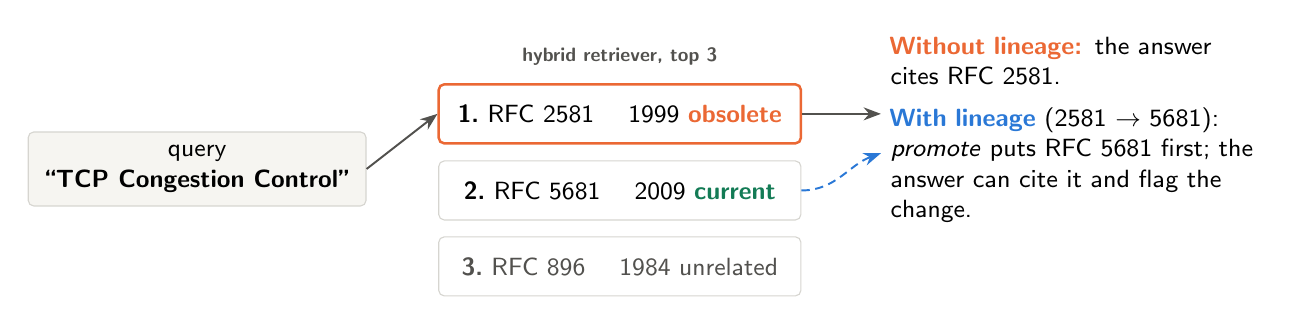
\begin{tikzpicture}[font=\sffamily\small, node distance=4mm,
  doc/.style={draw=rule, fill=white, rounded corners=2pt, minimum width=46mm,
    minimum height=7.5mm, align=left, inner sep=4pt},
  arr/.style={-{Stealth[length=2.2mm]}, ink2, line width=0.7pt}]
\node[draw=rule, fill=paper, rounded corners=2pt, inner sep=5pt, align=center] (q)
  {query\\\textbf{``TCP Congestion Control''}};
\node[right=9mm of q, yshift=7mm, doc, draw=orange, line width=0.9pt] (d1)
  {\textbf{1.}\ RFC 2581 \quad 1999 \hfill\textcolor{orange}{\textbf{obsolete}}};
\node[below=2mm of d1, doc] (d2)
  {\textbf{2.}\ RFC 5681 \quad 2009 \hfill\textcolor{aqua!70!black}{\textbf{current}}};
\node[below=2mm of d2, doc, text=ink2] (d3) {\textbf{3.}\ RFC 896 \quad 1984 \hfill unrelated};
\node[above=1mm of d1, font=\sffamily\scriptsize\bfseries, text=ink2] {hybrid retriever, top 3};
\draw[arr] (q.east) -- (d1.west);
\node[right=10mm of d1, yshift=-2mm, align=left, text width=46mm, font=\sffamily\small] (fix)
  {\textcolor{orange}{\textbf{Without lineage:}} the answer cites RFC 2581.\\[4pt]
   \textcolor{blue}{\textbf{With lineage}} (2581 $\rightarrow$ 5681): \emph{promote} puts
   RFC 5681 first; the answer can cite it and flag the change.};
\draw[arr] (d1.east) -- (fix.west|-d1.east);
\draw[arr, blue, densely dashed] (d2.east) to[out=0, in=200] ([yshift=-3mm]fix.west);
\end{tikzpicture}
\caption{A real ranking from the benchmark. RFC 5681 replaced RFC 2581 in 2009, but
the hybrid retriever ranks the obsolete document first. The same happens for
TLS~1.2: the current version, RFC~9846, only comes fourth, behind two documents it
replaced.}
\label{fig:problem}
\end{figure}

We ask three questions:
\begin{enumerate}[label=\textbf{Q\arabic*.}, leftmargin=2.4em]
\item How often does retrieval surface the obsolete version first? (§\ref{sec:retrieval})
\item Does it reach the generated answer, and can an answer policy contain it? (§\ref{sec:answers})
\item When lineage is not recorded, can we infer it, cheaply and with an agent? (§\ref{sec:librarian}–\ref{sec:agent})
\end{enumerate}

\begin{tcolorbox}[enhanced,colback=paper,colframe=paper,arc=2pt,left=8pt,right=8pt,
  top=5pt,bottom=5pt,title={\sffamily\bfseries\small How to read the numbers},
  coltitle=ink,colbacktitle=paper,fontupper=\small]
\begin{tabular}{@{}p{0.22\linewidth}p{0.72\linewidth}@{}}
\textbf{stale@1} & share of queries whose \emph{top} result is an obsolete version (lower is better).\\
\textbf{current@1} & share of queries whose top result is a version in force (higher is better).\\
\textbf{lineage} & the graph of which document replaces which. \emph{Oracle} lineage is the true one, from the index.\\
\textbf{gap closed} & how much of the improvement from no lineage to oracle lineage an inferred lineage recovers.\\
\textbf{balanced accuracy} & the mean of the hit rate on true replacements and on non-replacements; 0.5 is chance.\\
\textbf{[a, b]} & a 95\% bootstrap confidence interval. Overlapping intervals mean the difference is not established.\\
\end{tabular}
\end{tcolorbox}

% =========================================================================
\section{The benchmark}\label{sec:bench}
\final[final · RFC snapshot \res{corpus.sha}]

\paragraph{Documents and lineage} We parse the RFC index (\code{rfc-index.xml},
built \res{corpus.built}): \res{corpus.n_docs} RFCs, each with a title, year,
keywords and, for \res{corpus.n_docs_with_abstract} of them, an abstract. The
index records \emph{obsoletes} and \emph{obsoleted-by}; taking a link from either
side gives \res{corpus.n_supersession_edges} replacement links over
\res{corpus.n_superseded_docs} obsolete documents, forming
\res{corpus.n_components} lineages (the largest has
\res{corpus.max_component_size} documents). The \emph{current versions} of a
document are the ends of its chain of replacements; a split can produce several.
\emph{Updates} relations (\res{corpus.n_update_edges}) amend a document without
replacing it and are not used as ground truth.

\paragraph{Splits} All queries and pairs of one lineage share a split (30\% dev,
70\% test), so no lineage is seen on both sides.

\paragraph{Title queries} For each link, the old title and the new title are each
used as a query: \res{corpus.n_queries} queries (\res{corpus.n_queries.test} test).
Any current version is a correct result; any obsolete member of the lineage is stale.

\paragraph{Change-aware questions} Title queries are artificial, so we also
generate natural questions whose answer \emph{changed} between versions. For
\res{qgen.attempted} sampled links, an LLM reads both abstracts and writes a
question, the old and new answers, and verbatim evidence from each. Automatic
checks reject evidence that is not verbatim, questions that name an RFC or give
away the answer, and answers argued from silence. \res{qgen.accepted} questions
pass (\res{qgen.rate}); in \res{qgen.skipped} cases the model found no
substantive change and declined (Table~\ref{tab:qgen} in the appendix).

The benchmark is public on Hugging Face (\S\ref{sec:repro}).

% =========================================================================
\section{Q1: does retrieval surface the obsolete version?}\label{sec:retrieval}
\final

\paragraph{Setup} Three retrievers: BM25~\cite{robertson2009bm25}, dense
embeddings (\code{bge-small-en-v1.5}~\cite{xiao2023cpack}), and their reciprocal
rank fusion~\cite{cormack2009rrf} (``hybrid''). Top 10. With oracle lineage we also
test two fixes: \code{filter} drops obsolete documents; \code{promote} replaces each
obsolete hit with its current version, at the same rank.

\begin{figure}[t]
\centering
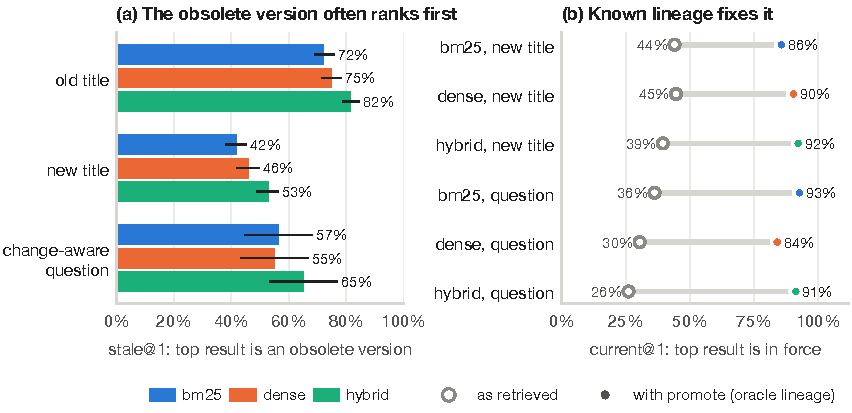
\includegraphics[width=\linewidth]{generated/fig_retrieval.pdf}
\caption{\textbf{(a)} Share of queries whose top result is obsolete, by query type
and retriever, with 95\% intervals. \textbf{(b)} Share whose top result is current,
as retrieved (hollow) and after \code{promote} with oracle lineage (filled).
Test split; questions use all splits ($n{=}\res{qret.n}$). Full numbers:
Tables~\ref{tab:retrieval}–\ref{tab:qretrieval}.}
\label{fig:retrieval}
\end{figure}

\paragraph{Results} Every retriever often ranks the obsolete version first
(Fig.~\ref{fig:retrieval}a): on new-title queries, \res{ret.bm25.new_title.none.stale1.pct}
of the time with BM25, \res{ret.dense.new_title.none.stale1.pct} with dense retrieval and
\res{ret.hybrid.new_title.none.stale1.pct} with the hybrid; on change-aware questions,
\res{qret.hybrid.none.stale1.pct} \res{qret.hybrid.none.stale1.cipct} with the hybrid.
The best topical matcher is the most stale, because the old document \emph{is} a
good match for the topic, as HoH found for dense retrievers on
Wikipedia~\cite{ouyang2025hoh}. With oracle lineage, \code{promote} raises the hybrid's
current@1 from \res{ret.hybrid.new_title.none.current1.pct} to
\res{ret.hybrid.new_title.promote.current1.pct} on new titles
(Fig.~\ref{fig:retrieval}b).

\paragraph{Is newest-first enough?} A fix without lineage is to prefer recent
documents. We re-rank the hybrid's top 50 by year within a window
(\code{newest\_first}) or by score $\times\,e^{-\lambda\cdot\text{age}}$
(\code{time\_decay}, as in HoH~\cite{ouyang2025hoh}), with the window and
$\lambda$ tuned on dev. With correct years, this halves staleness but stops well
short of lineage: on new-title queries the hybrid's current@1 rises from
\res{ret.hybrid.new_title.none.current1.pct} to
\res{ret.hybrid.new_title.newest_first.current1.pct} (newest-first) and
\res{ret.hybrid.new_title.time_decay.current1.pct} (time decay), against
\res{ret.hybrid.new_title.promote.current1.pct} with \code{promote}; on
questions, \res{qret.hybrid.newest_first.current1.pct} against
\res{qret.hybrid.promote.current1.pct}. A newer document is not necessarily the
replacement: it may be an unrelated, companion or partial update. Recency also
needs correct years, which Section~\ref{sec:noise} relaxes.

\Takeaway{Staleness is a property of the collection, not of a weak retriever:
better retrieval makes it worse. Knowing the lineage removes it almost completely,
which is why the rest of the paper is about recovering the lineage.}

% =========================================================================
\section{Q2: does it reach the answer?}\label{sec:answers}
\final[final · human check of the judge pending]

\paragraph{Setup} For each question, the hybrid retriever's results go to an
answering model (\code{\res{ans.answer_model}}, top \res{ans.context_k}) under
three policies, all using oracle lineage except the first:
\code{naive} (context as retrieved); \code{latest\_only} (current versions only);
\code{show\_conflict} (\code{promote} order, obsolete documents kept and marked as
replaced). A judge model (\code{\res{ans.judge_model}}) compares each answer with
the reference old and new answers. A \emph{stale} outcome gives the old answer
without flagging it as outdated.

In the standard context each passage shows its year and RFC number, which a
strong model can use to pick the newer one by itself. The \emph{blind} variant
hides years and numbers, as in collections without reliable metadata.

\begin{figure}[t]
\centering
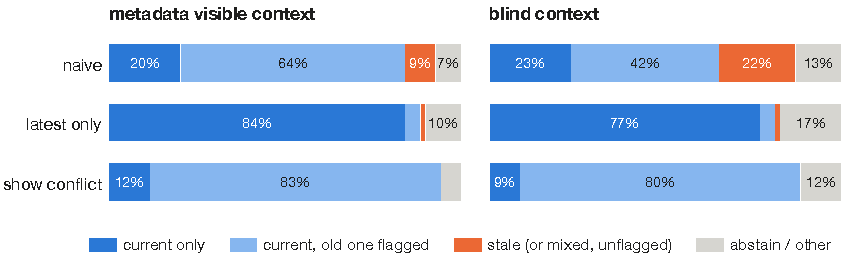
\includegraphics[width=\linewidth]{generated/fig_answers.pdf}
\caption{What the answers say, per policy ($n{=}\res{ans.n}$ questions each).
``Current, old one flagged'' gives the new answer and mentions the old one as
outdated. Table~\ref{tab:answers} in the appendix gives intervals.}
\label{fig:answers}
\end{figure}

\paragraph{Results} With metadata visible, \code{naive} gives a stale answer
\res{ans.std.naive.stale_outcome} of the time; the model mostly resolves versions
itself. Blind, this rises to \res{ans.blind.naive.stale_outcome}
\res{ans.blind.naive.stale_outcome.ci} (Fig.~\ref{fig:answers}).
\code{show\_conflict} keeps it at \res{ans.blind.show_conflict.stale_outcome}
and gives the most current answers (\res{ans.blind.show_conflict.current_outcome}
blind), while telling the reader what changed.

\paragraph{What the model knows without documents} Asked the same questions with no documents,
the answering model gives the current answer \res{cb.current} of the time
\res{cb.current.ci} and the old one \res{cb.stale}: it has read most of these RFCs.
So retrieval does not supply knowledge the model lacks; it \emph{overrides}
knowledge the model has. Of the \res{cb.blind.naive.override.n} questions it gets
right closed-book, blind \code{naive} RAG turns \res{cb.blind.naive.override.k}
(\res{cb.blind.naive.override}) into stale answers
(\res{cb.standard.naive.override} with metadata visible); \code{latest\_only} and
\code{show\_conflict} turn none. Where it does not know (\res{cb.blind.naive.rescue.n}
questions), current documents rescue it, \res{cb.blind.show_conflict.rescue} of
the time with \code{show\_conflict} blind. This is a lower bound for less familiar
collections, such as internal procedures, which no model has read.

\paragraph{Judge reliability} A second model labelled \res{judge.model.n}
answers without seeing the judge's labels: Cohen's
$\kappa=\res{judge.model.kappa}$~\cite{cohen1960kappa} (\res{judge.model.agree} of
\res{judge.model.n} identical). This is agreement between two models; a human
check is pending ($\kappa=\res{judge.human.kappa}$, $n=\res{judge.human.n}$).

\Takeaway{Where metadata is missing, about one answer in five is stale, often
where the model knew better without retrieval. Showing both versions, with the old
one marked, fixes it, but it needs the lineage.}

% =========================================================================
\section{Q3a: inferring lineage cheaply}\label{sec:librarian}
\final[final · librarian v0]

\paragraph{Hiding the answer} Many abstracts say outright ``This document
obsoletes RFC 2581'', and the index's lineage fields are hidden from every method.
Three settings: \code{declared} keeps the text; \code{masked} replaces every RFC
number with a neutral token; \code{strict} also removes sentences that announce a
replacement. \code{strict} matches collections that never declare it.

\paragraph{Method} Candidate pairs are each document's 10 nearest neighbours by
abstract and by title embedding, older first (\res{lin.strict.ncand} pairs, covering
\res{lin.strict.recall.pct} of the true links). Each pair gets cheap features (title and
abstract similarity, year gap, version cues such as ``bis'' or ``version 2'',
shared keywords, neighbour rank) and a score from a logistic regression trained on
the dev split, with a threshold chosen on dev. Each old document keeps its best
replacement above the threshold. As a learning-free baseline in the style of
Modani et al.~\cite{modani2021versions}, \emph{version chains} link candidate pairs
whose title or abstract similarity exceeds a threshold (tuned on dev), treat each
connected group as a version family, and chain its members in publication order.

\begin{figure}[t]
\centering
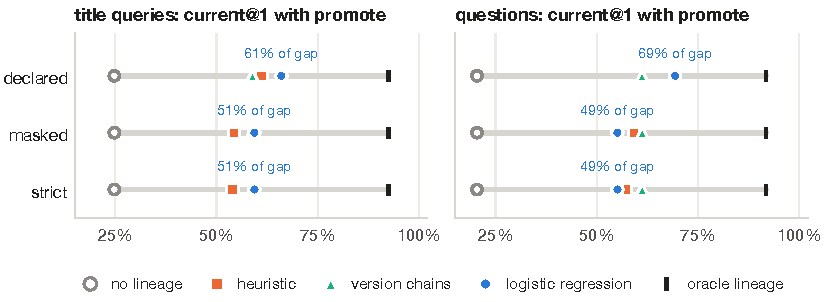
\includegraphics[width=\linewidth]{generated/fig_lineage.pdf}
\caption{current@1 after \code{promote} using inferred lineage, between no lineage
(hollow) and oracle lineage (bar); squares: heuristic, triangles: version chains,
dots: logistic regression. Labels: share of the gap closed by the logistic
regression. Edge precision, recall and F1 in Table~\ref{tab:lineage}.}
\label{fig:lineage}
\end{figure}

\paragraph{Results} The logistic regression's edge F1 drops from
\res{lin.declared.logreg.f1} (declared) to \res{lin.strict.logreg.f1} (strict),
while version chains hold at \res{lin.strict.version_chains.f1}: once explicit cues
are gone, the learned scorer is no better than clustering similar documents.
Downstream the two are close: \res{lin.strict.logreg.title.gap} and
\res{lin.strict.version_chains.title.gap} of the gap closed on title queries,
\res{lin.strict.logreg.questions.gap} and \res{lin.strict.version_chains.questions.gap}
on questions (Fig.~\ref{fig:lineage}). Its mistakes cluster in a band of high but uncertain
scores, mostly pairs with near-identical titles that are companions rather than
successors.

\Takeaway{Cheap signals recover half of what lineage is worth, about as much as
preferring recent documents (Section~\ref{sec:noise}). The other half sits in
ambiguous pairs that need reading, which is the agent's job.}

% =========================================================================
\section{When years are missing or wrong}\label{sec:noise}
\final

\paragraph{Setup} Recency baselines need correct years, and so does our cheap
scorer, which uses years to orient a pair (older$\to$newer) and as a feature. We
remove or shift (by 1--10 years) the year of a random share of documents, re-tune
the recency parameters, and re-fit the scorer on the corrupted data, over
\res{noise.seeds} seeds per level. Document numbers are never used for ordering,
so they cannot leak the true order. Oracle lineage needs no years and is the
ceiling.

\begin{figure}[t]
\centering
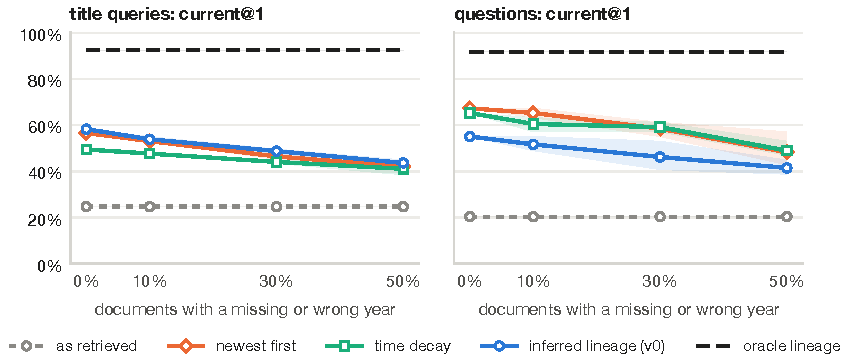
\includegraphics[width=\linewidth]{generated/fig_noise.pdf}
\caption{current@1 of the hybrid's top 10 on test queries as a growing share of
years is removed or shifted. Lines are means over seeds; bands span the seeds.
Inferred lineage uses the \code{strict} setting.}
\label{fig:noise}
\end{figure}

\paragraph{Results} With correct years, newest-first reaches
\res{noise.title.newest_first.0.current1} current@1 on title queries and the
inferred lineage \res{noise.title.lineage_v0.0.current1}. With half of the years
missing or wrong, newest-first falls to \res{noise.title.newest_first.50.current1}
and time decay to \res{noise.title.time_decay.50.current1}, while the inferred
lineage keeps \res{noise.title.lineage_v0.50.current1}
(Fig.~\ref{fig:noise}); on questions the corresponding values are
\res{noise.questions.newest_first.50.current1},
\res{noise.questions.time_decay.50.current1} and
\res{noise.questions.lineage_v0.50.current1}.

\Takeaway{The cheap scorer is \emph{not} more robust than recency: it orients pairs by
year, so it degrades at the same rate, and with correct years simple recency
already matches it (title queries) or beats it (questions). Both stay far below
oracle lineage at every noise level. Closing that gap needs judgements made from
the content, which is what the agent is for; whether the agent holds up when years
are wrong is the next test.}

% =========================================================================
\section{Q3b: a librarian agent for the uncertain cases}\label{sec:agent}
\prelim[100 pairs · repeats, second model and downstream effect pending]

\paragraph{Design} The agent decides whether a newer document replaces an older
one (Fig.~\ref{fig:agentdiagram}). It is a LangGraph state machine: \emph{triage}
settles pairs the cheap scorer is sure about; \emph{investigate} lets the model call
tools for up to 8 steps, ReAct-style~\cite{yao2023react}; \emph{decide} returns a
structured verdict (\emph{supersedes}, \emph{amends}, \emph{conflicts},
\emph{unrelated}) with a confidence and a one-line rationale. The tools come from
an MCP server, the same one used in deployment, and never reveal lineage:
\code{search}, \code{read\_doc}, \code{compare} and \code{find\_later} (documents on
the same topic published later: the candidate replacements). Models run locally
through Ollama at temperature 0.

\begin{figure}[t]
\centering
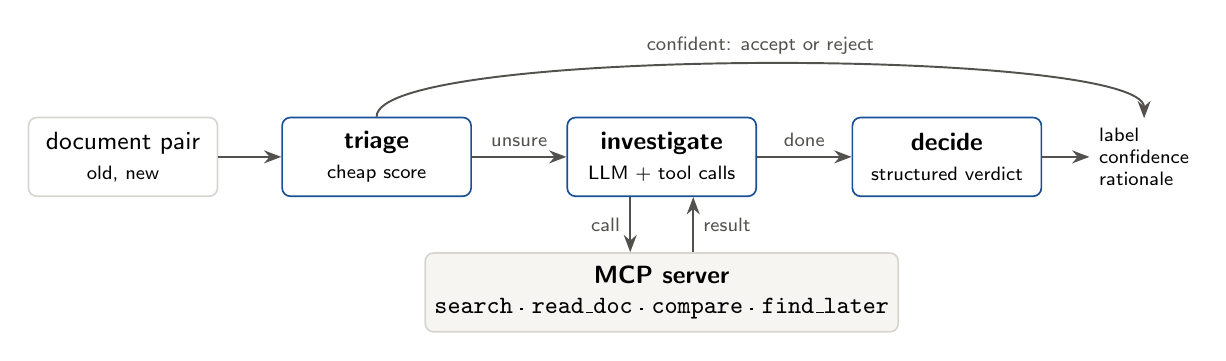
\begin{tikzpicture}[font=\sffamily\small, node distance=5mm and 8mm,
  box/.style={draw=rule, fill=white, rounded corners=3pt, minimum height=10mm,
    minimum width=24mm, align=center, line width=0.6pt},
  arr/.style={-{Stealth[length=2.2mm]}, ink2, line width=0.7pt},
  lab/.style={font=\sffamily\scriptsize, text=ink2}]
\node[box] (pair) {document pair\\\scriptsize old, new};
\node[box, right=of pair, draw=accent] (triage) {\textbf{triage}\\\scriptsize cheap score};
\node[box, right=12mm of triage, draw=accent] (inv) {\textbf{investigate}\\\scriptsize LLM + tool calls};
\node[box, right=12mm of inv, draw=accent] (decide) {\textbf{decide}\\\scriptsize structured verdict};
\node[box, below=7mm of inv, fill=paper, minimum width=56mm] (tools)
  {\textbf{MCP server}\\\scriptsize\code{search} · \code{read\_doc} · \code{compare} · \code{find\_later}};
\node[right=6mm of decide, align=left, font=\sffamily\scriptsize] (out)
  {label\\confidence\\rationale};
\draw[arr] (pair) -- (triage);
\draw[arr] (triage) -- node[lab, above]{unsure} (inv);
\draw[arr] (inv) -- node[lab, above]{done} (decide);
\draw[arr] (decide) -- (out);
\draw[arr] ([xshift=-4mm]inv.south) -- node[lab, left]{call} ([xshift=-4mm]tools.north);
\draw[arr] ([xshift=4mm]tools.north) -- node[lab, right]{result} ([xshift=4mm]inv.south);
\draw[arr] (triage.north) .. controls +(0,9mm) and +(0,9mm) .. node[lab, above]{confident: accept or reject} (out.north);
\end{tikzpicture}
\caption{The librarian agent. Only pairs in the cheap scorer's uncertain band reach
the language model, so the agent's cost scales with ambiguity, not corpus size.}
\label{fig:agentdiagram}
\end{figure}

\paragraph{Evaluation} We take test pairs whose cheap-scorer probability falls in the
uncertain band \res{ag.band} (\code{strict} setting, \res{ag.bandsize} pairs) and
draw a seeded sample of \res{ag.n}: \res{ag.half} true replacements and \res{ag.half}
non-replacements. The sample is nested (its first 20 and 50 pairs are the samples
used for repeated runs). Each method is scored \emph{on the same pairs}, against
two ground truths: \emph{strict} (the index records the link directly) and
\emph{lineage} (a later version through a chain also counts: if A$\to$B$\to$C, then
``C replaces A'' is right for a reader). The sample is balanced but the band is
not (\res{ag.prior.strict.pct} of band pairs are true links), so we report the
precision expected in use, estimated from the hit rates (Table~\ref{tab:agent}).
Paired differences are tested with an exact McNemar test and a paired bootstrap of
the balanced-accuracy difference.

\paragraph{What we compare} Three ways of using the same model
(\code{qwen3.5}, 9.7B, temperature 0) and the same prompt (v2), to tell what the
tools add: \emph{LLM only} reads both documents (the same text \code{read\_doc}
returns) and decides in one call; \emph{agent without \code{find\_later}} has
\code{search}, \code{read\_doc} and \code{compare}; \emph{agent, all tools} adds
\code{find\_later}. The cheap scorer uses its own tuned threshold
(\res{ag.threshold}). Prompt v2 was written after looking at 20 earlier pairs, ten
of which are in this sample (Appendix~\ref{sec:agentruns}).

\begin{figure}[t]
\centering
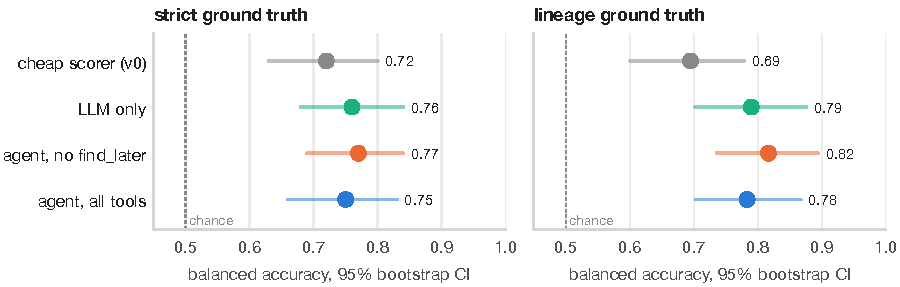
\includegraphics[width=\linewidth]{generated/fig_agent.pdf}
\caption{Balanced accuracy on the same \res{ag.n} band pairs, with 95\% stratified
bootstrap intervals. Grey: the cheap scorer; colours: the same Qwen~3.5 model
with no tools (aqua), three tools (orange) and all four tools (blue); hollow:
Ministral~3 with all tools.}
\label{fig:agent}
\end{figure}

\paragraph{Results} All three model-based methods do somewhat better than the
cheap scorer, and none of the differences is significant (Fig.~\ref{fig:agent}).
Under the strict ground truth, the full agent reaches
\res{ag.qwen3.5-hermes.full.strict.ba} \res{ag.qwen3.5-hermes.full.strict.ba.ci}
against \res{ag.cheap.strict.ba} \res{ag.cheap.strict.ba.ci} (difference
\res{ag.pair.qwen3.5-hermes.full.cheap.strict.diff}
\res{ag.pair.qwen3.5-hermes.full.cheap.strict.diff.ci}, McNemar
$p=\res{ag.pair.qwen3.5-hermes.full.cheap.strict.p}$). Under the lineage ground
truth the gap widens: the agent without \code{find\_later} reaches
\res{ag.qwen3.5-hermes.no_find_later.lineage.ba} against
\res{ag.cheap.lineage.ba} (McNemar
$p=\res{ag.pair.qwen3.5-hermes.no_find_later.cheap.lineage.p}$). Many of the
model's ``false'' replacements are later issues of the same series, such as two
editions of \emph{Internet Official Protocol Standards} several versions apart:
wrong for the index, right for a reader.

The tools do not help. A single call without tools
(\res{ag.qwen3.5-hermes.llm_only.strict.ba}) is as accurate as the full agent
(difference \res{ag.pair.qwen3.5-hermes.full.qwen3.5-hermes.llm_only.strict.diff},
$p=\res{ag.pair.qwen3.5-hermes.full.qwen3.5-hermes.llm_only.strict.p}$) at a quarter
of the cost: \res{ag.qwen3.5-hermes.llm_only.seconds}~s per pair against
\res{ag.qwen3.5-hermes.full.seconds}~s, and
\res{ag.qwen3.5-hermes.llm_only.intok} input tokens against
\res{ag.qwen3.5-hermes.full.intok} (Fig.~\ref{fig:agentcost},
Table~\ref{tab:agentcost}). The two make the same call on most pairs. The agent
does follow the procedure (it calls \code{compare} and \code{find\_later} on every
pair), but what it finds rarely changes its mind.

A second model, Ministral~3 (8B) with the same prompt and all tools, lands in the
same place: \res{ag.ministral-3.full.strict.ba} \res{ag.ministral-3.full.strict.ba.ci}
(McNemar against the scorer
$p=\res{ag.pair.ministral-3.full.cheap.strict.p}$), at
\res{ag.ministral-3.full.seconds}~s per pair. It calls \code{compare} on every pair
and never \code{find\_later}, so it decides from the two documents alone, like the
no-tool variant.

All model-based methods say ``replaces'' too readily: the full agent does so on
\res{ag.qwen3.5-hermes.full.yes} of a balanced sample, with true-positive rate
\res{ag.qwen3.5-hermes.full.strict.tpr} and true-negative rate
\res{ag.qwen3.5-hermes.full.strict.tnr}. In the real band, where only
\res{ag.prior.strict.pct} of pairs are true links, this gives an expected precision
of \res{ag.qwen3.5-hermes.full.strict.prec}, below the scorer's
\res{ag.cheap.strict.prec}. Whether the extra recall outweighs the extra false
links downstream is what the cascade experiment measures (pending).

\begin{figure}[t]
\centering
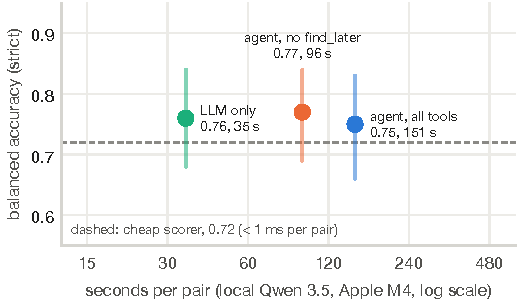
\includegraphics[width=0.66\linewidth]{generated/fig_agent_cost.pdf}
\caption{Accuracy against cost per pair on a laptop (Apple M4). Bars: 95\%
bootstrap intervals; hollow: Ministral~3. The dashed line is the cheap scorer.}
\label{fig:agentcost}
\end{figure}

\Takeaway{On pairs where cheap signals are ambiguous, reading the two documents
helps a little, mostly by recognising later versions in a chain; the investigation
tools add cost but no accuracy. A tool-using agent is not yet justified over a
single model call here. Next: repeated runs, a second model, the effect on
retrieval through the cascade, and whether reading holds up when years are wrong,
where the cheap scorer and recency both fail (§\ref{sec:noise}).}

% =========================================================================
\section{Related work}\label{sec:related}

\paragraph{Outdated documents in RAG} HoH~\cite{ouyang2025hoh} builds 96k
questions from monthly Wikipedia diffs, keeps current and outdated passages
together, and shows that outdated passages hurt more than distracting ones and
that stronger retrievers fetch more of them; mitigations rely on modification
times. Stale-Document Poisoning~\cite{ahmed2026poisoning} measures how often
outdated evidence overturns an answer a model gets right closed-book (17--91\% for
open models, 317 reversals in four domains); its recency re-ranker helps only when
dates are correct, and with wrong dates it stops selecting the current document
at all. MemStrata~\cite{memstrata2026} retires superseded facts in agent memory
using ingestion order as time, and warns that textual markers such as
``deprecated'' let baselines read the answer, which our masked and strict
settings rule out. ChurnBench~\cite{singh2026churnbench} measures freshness errors
of agents over enterprise data with timestamped change logs. All of these assume
time metadata or change logs; \emph{we target collections where lineage is
unrecorded and dates are unreliable}, and infer the lineage.

\paragraph{Version detection} Modani et al.~\cite{modani2021versions} detect
versions and order them in a Wikipedia-derived collection. GVD~\cite{sediqin2026gvd}
groups enterprise documents into version families and classifies rule-level
relations (duplicate, contradiction, refinement) without an LLM, on 120
confidential documents, without a downstream RAG evaluation. We infer directed
replacement links, including chains, on a public benchmark, and measure their
effect on retrieval and answers; our second stage is an agent with tools.

\paragraph{Knowledge conflicts and time} Conflict benchmarks such as
ConflictBank~\cite{su2024conflictbank} and WikiContradict~\cite{hou2024wikicontradict}
study disagreements between memory and context or between passages;
time-sensitive QA~\cite{chen2021timeqa,kasai2023realtimeqa,dhingra2022timeaware}
studies questions whose answer changes; and knowledge-conflict work asks how models
arbitrate~\cite{longpre2021entity,xie2024chameleon}. Here the conflict has a ground
truth, the lineage. LLM judges~\cite{zheng2023judge} need validation, which we
report as agreement statistics; the agent follows the ReAct pattern of interleaved
reasoning and tool calls~\cite{yao2023react}.

\section{Limitations and next steps}
\begin{itemize}
\item \textbf{One domain.} RFCs, with short abstracts. Aviation advisory
  circulars are next. The answering model knows the current answer to
  \res{cb.current} of the questions without documents (§\ref{sec:answers});
  collections no model has read will test retrieval harder.
\item \textbf{Few questions, model-checked.} \res{qgen.accepted} change-aware
  questions, validated against a second model rather than people (a human check
  is pending; HoH and Stale-Document Poisoning report human checks). A larger,
  head-only generation is planned.
\item \textbf{One answering model} so far; open-weight answering models are in
  progress.
\item \textbf{Agent evidence is limited.} One model, one prompt, \res{ag.n} pairs:
  the intervals are about $\pm$0.08 wide, so differences under 0.1 are not
  detectable. Repeated runs, a second model, the downstream effect and the
  year-noise condition are in progress.
\item \textbf{Deployment.} The serving code (HTTP search with inferred lineage, the
  cascade, MCP and A2A interfaces) is in the repository; the cloud deployment is in progress and
  will be reported with latency and cost.
\end{itemize}

\section{Reproducibility and release}\label{sec:repro}
Code, results and this paper: \url{https://github.com/CarlHatoum/supersede}.
\code{make paper} regenerates every number, table and figure from \code{results/}.
LLM calls for questions, answers and judging are cached, so \code{make reproduce}
rebuilds them offline; agent decisions are logged per pair with tool traces.
The benchmark is at \url{https://huggingface.co/datasets/hatoum/supersede-rfc}.
RFC abstracts ship verbatim, as the IETF Trust Legal Provisions allow unmodified,
attributed excerpts but not modified text; the \code{masked} and \code{strict} views
are derived locally by a script shipped with the data.

% =========================================================================
\clearpage
\appendix
\section{Full tables}

\begin{table}[H]
\centering\small
\begin{tabular}{lllrrrr}
\toprule
retriever & query & policy & stale@1$\downarrow$ & current@1$\uparrow$ & current@10$\uparrow$ & MRR$\uparrow$ \\
\midrule
bm25 & new title & \texttt{none} & 0.417 & 0.440 & 0.931 & 0.628 \\
 &  & \texttt{filter} & 0.000 & 0.750 & 0.931 & 0.821 \\
 &  & \texttt{promote} & 0.000 & 0.857 & 0.983 & 0.905 \\
 &  & \texttt{newest\_first} & 0.161 & 0.590 & 0.931 & 0.703 \\
 &  & \texttt{time\_decay} & 0.124 & 0.579 & 0.906 & 0.704 \\
 & old title & \texttt{none} & 0.722 & 0.152 & 0.790 & 0.394 \\
 &  & \texttt{filter} & 0.000 & 0.568 & 0.790 & 0.651 \\
 &  & \texttt{promote} & 0.000 & 0.874 & 0.986 & 0.916 \\
 &  & \texttt{newest\_first} & 0.274 & 0.448 & 0.790 & 0.542 \\
 &  & \texttt{time\_decay} & 0.352 & 0.357 & 0.778 & 0.508 \\
\midrule
dense & new title & \texttt{none} & 0.459 & 0.446 & 0.928 & 0.643 \\
 &  & \texttt{filter} & 0.000 & 0.803 & 0.928 & 0.855 \\
 &  & \texttt{promote} & 0.000 & 0.904 & 0.992 & 0.938 \\
 &  & \texttt{newest\_first} & 0.186 & 0.670 & 0.928 & 0.756 \\
 &  & \texttt{time\_decay} & 0.140 & 0.609 & 0.913 & 0.720 \\
 & old title & \texttt{none} & 0.749 & 0.170 & 0.793 & 0.415 \\
 &  & \texttt{filter} & 0.000 & 0.620 & 0.793 & 0.686 \\
 &  & \texttt{promote} & 0.000 & 0.916 & 0.996 & 0.947 \\
 &  & \texttt{newest\_first} & 0.321 & 0.496 & 0.793 & 0.578 \\
 &  & \texttt{time\_decay} & 0.321 & 0.384 & 0.774 & 0.517 \\
\midrule
hybrid & new title & \texttt{none} & 0.528 & 0.395 & 0.937 & 0.621 \\
 &  & \texttt{filter} & 0.000 & 0.809 & 0.937 & 0.861 \\
 &  & \texttt{promote} & 0.000 & 0.923 & 0.994 & 0.950 \\
 &  & \texttt{newest\_first} & 0.183 & 0.653 & 0.937 & 0.750 \\
 &  & \texttt{time\_decay} & 0.169 & 0.597 & 0.941 & 0.737 \\
 & old title & \texttt{none} & 0.816 & 0.111 & 0.810 & 0.389 \\
 &  & \texttt{filter} & 0.000 & 0.615 & 0.810 & 0.689 \\
 &  & \texttt{promote} & 0.000 & 0.927 & 0.996 & 0.953 \\
 &  & \texttt{newest\_first} & 0.315 & 0.486 & 0.810 & 0.576 \\
 &  & \texttt{time\_decay} & 0.327 & 0.401 & 0.820 & 0.556 \\
\bottomrule
\end{tabular}

\caption{Retrieval on test-split title queries ($n{=}\res{ret.new_title.n}$ new-title,
\res{ret.old_title.n} old-title). \code{filter} and \code{promote} use oracle lineage.}
\label{tab:retrieval}
\end{table}

\begin{table}[H]
\centering\small
\begin{tabular}{llll}
\toprule
retriever & policy & stale@1$\downarrow$ [95\% CI] & current@1$\uparrow$ \\
\midrule
bm25 & \texttt{none} & 0.565 [0.449, 0.681] & 0.362 [0.261, 0.478] \\
 & \texttt{filter} & 0.000 [0.000, 0.000] & 0.768 [0.667, 0.870] \\
 & \texttt{promote} & 0.000 [0.000, 0.000] & 0.928 [0.870, 0.986] \\
\midrule
 & \texttt{newest\_first} & 0.217 [0.116, 0.319] & 0.609 [0.493, 0.725] \\
 & \texttt{time\_decay} & 0.174 [0.087, 0.275] & 0.638 [0.522, 0.754] \\
dense & \texttt{none} & 0.551 [0.435, 0.667] & 0.304 [0.203, 0.420] \\
\midrule
 & \texttt{filter} & 0.000 [0.000, 0.000] & 0.681 [0.565, 0.783] \\
 & \texttt{promote} & 0.000 [0.000, 0.000] & 0.841 [0.754, 0.913] \\
 & \texttt{newest\_first} & 0.188 [0.101, 0.275] & 0.623 [0.507, 0.739] \\
 & \texttt{time\_decay} & 0.101 [0.043, 0.174] & 0.609 [0.493, 0.725] \\
hybrid & \texttt{none} & 0.652 [0.536, 0.768] & 0.261 [0.159, 0.362] \\
 & \texttt{filter} & 0.000 [0.000, 0.000] & 0.783 [0.681, 0.870] \\
 & \texttt{promote} & 0.000 [0.000, 0.000] & 0.913 [0.841, 0.971] \\
 & \texttt{newest\_first} & 0.188 [0.101, 0.275] & 0.681 [0.565, 0.783] \\
 & \texttt{time\_decay} & 0.145 [0.072, 0.232] & 0.667 [0.551, 0.783] \\
\bottomrule
\end{tabular}

\caption{Retrieval on change-aware questions ($n{=}\res{qret.n}$, all splits).}
\label{tab:qretrieval}
\end{table}

\begin{table}[H]
\centering\small
\begin{tabular}{lllrrr}
\toprule
context & policy & stale answer$\downarrow$ [95\% CI] & current$\uparrow$ & conflict flagged & abstain \\
\midrule
standard & \texttt{naive} & 8.7\% [2.9\%, 15.9\%] & 84.1\% & 63.8\% & 5.8\% \\
 & \texttt{latest\_only} & 1.4\% [0.0\%, 4.3\%] & 88.4\% & 4.3\% & 7.2\% \\
 & \texttt{show\_conflict} & 0.0\% [0.0\%, 0.0\%] & 94.2\% & 82.6\% & 4.3\% \\
\midrule
blind & \texttt{naive} & 21.7\% [13.0\%, 31.9\%] & 65.2\% & 42.0\% & 13.0\% \\
 & \texttt{latest\_only} & 1.4\% [0.0\%, 4.3\%] & 81.2\% & 4.3\% & 14.5\% \\
 & \texttt{show\_conflict} & 0.0\% [0.0\%, 0.0\%] & 88.4\% & 79.7\% & 10.1\% \\
\bottomrule
\end{tabular}

\caption{Answer outcomes ($n{=}\res{ans.n}$), hybrid retrieval,
top-\res{ans.context_k} context. ``Current'' includes answers that flag the old version.}
\label{tab:answers}
\end{table}

\begin{table}[H]
\centering\small
\resizebox{\linewidth}{!}{\begin{tabular}{llrrrrr}
\toprule
setting & method & edge P & edge R & edge F1 & title queries: current@1 (gap) & questions: current@1 (gap) \\
\midrule
declared & no lineage & -- & -- & -- & 0.248 (0\%) & 0.204 (0\%) \\
 & heuristic & 0.325 & 0.541 & 0.406 & 0.612 (54\%) & 0.694 (69\%) \\
 & logreg & 0.775 & 0.578 & 0.663 & 0.660 (61\%) & 0.694 (69\%) \\
 & oracle & -- & -- & -- & 0.925 (100\%) & 0.918 (100\%) \\
\midrule
masked & no lineage & -- & -- & -- & 0.248 (0\%) & 0.204 (0\%) \\
 & heuristic & 0.288 & 0.449 & 0.351 & 0.543 (44\%) & 0.592 (54\%) \\
 & logreg & 0.593 & 0.481 & 0.531 & 0.594 (51\%) & 0.551 (49\%) \\
 & oracle & -- & -- & -- & 0.925 (100\%) & 0.918 (100\%) \\
\midrule
strict & no lineage & -- & -- & -- & 0.248 (0\%) & 0.204 (0\%) \\
 & heuristic & 0.286 & 0.444 & 0.348 & 0.539 (43\%) & 0.571 (51\%) \\
 & logreg & 0.596 & 0.492 & 0.539 & 0.594 (51\%) & 0.551 (49\%) \\
 & oracle & -- & -- & -- & 0.925 (100\%) & 0.918 (100\%) \\
\bottomrule
\end{tabular}
}
\caption{Lineage inference: edge scores on test pairs, and downstream current@1 with
\code{promote} (share of gap closed in brackets).}
\label{tab:lineage}
\end{table}

\begin{table}[H]
\centering\small
\begin{tabular}{llrrlrr}
\toprule
truth & method & TPR & TNR & bal. acc. [95\% CI] & est. prec. & s/pair \\
\midrule
strict & cheap scorer (v0) & 0.62 & 0.82 & 0.72 [0.63, 0.80] & 0.36 & -- \\
 & agent, all tools, \texttt{qwen3.5-hermes} & 0.84 & 0.66 & 0.75 [0.66, 0.83] & 0.29 & 151 \\
 & LLM only (no tools), \texttt{qwen3.5-hermes} & 0.88 & 0.64 & 0.76 [0.68, 0.84] & 0.29 & 35 \\
 & agent without \texttt{find\_later}, \texttt{qwen3.5-hermes} & 0.92 & 0.62 & 0.77 [0.69, 0.84] & 0.29 & 96 \\
\midrule
lineage & cheap scorer (v0) & 0.57 & 0.82 & 0.69 [0.60, 0.78] & 0.51 & -- \\
 & agent, all tools, \texttt{qwen3.5-hermes} & 0.84 & 0.73 & 0.78 [0.70, 0.87] & 0.50 & 151 \\
 & LLM only (no tools), \texttt{qwen3.5-hermes} & 0.88 & 0.70 & 0.79 [0.70, 0.88] & 0.49 & 35 \\
 & agent without \texttt{find\_later}, \texttt{qwen3.5-hermes} & 0.93 & 0.70 & 0.82 [0.74, 0.89] & 0.51 & 96 \\
\bottomrule
\end{tabular}

\caption{Agent variants and cheap scorer on the same \res{ag.n} band pairs.
Estimated precision uses the band's real share of true links
(\res{ag.prior.strict} strict, \res{ag.prior.lineage} lineage).}
\label{tab:agent}
\end{table}

\begin{table}[H]
\centering\small
\resizebox{\linewidth}{!}{\begin{tabular}{lrrrrrr}
\toprule
method & s/pair & model calls & tool calls & input tok. & output tok. & says replaces \\
\midrule
agent, all tools, \texttt{qwen3.5-hermes} & 151 & 4.0 & 2.0 & 5,437 & 803 & 59\% \\
LLM only (no tools), \texttt{qwen3.5-hermes} & 35 & 1.0 & 0.0 & 595 & 186 & 62\% \\
agent without \texttt{find\_later}, \texttt{qwen3.5-hermes} & 96 & 3.2 & 1.3 & 3,259 & 481 & 65\% \\
\bottomrule
\end{tabular}
}
\caption{Cost per pair (means; local Qwen~3.5 on an Apple M4) and the share of
pairs labelled ``replaces''.}
\label{tab:agentcost}
\end{table}

\begin{table}[H]
\centering\small
\begin{tabular}{lr}
\toprule
outcome & pairs \\
\midrule
\texttt{skipped\_by\_model} & 224 \\
\texttt{accepted} & 69 \\
\texttt{evidence\_current\_not\_verbatim} & 2 \\
\texttt{question\_leaks\_reference} & 2 \\
\texttt{answer\_from\_silence} & 1 \\
\texttt{evidence\_stale\_not\_verbatim} & 1 \\
\texttt{question\_reveals\_answer} & 1 \\
\bottomrule
\end{tabular}

\caption{Outcome of question generation per sampled link.}
\label{tab:qgen}
\end{table}

\clearpage
\section{Agent prompt development and traces}\label{sec:agentruns}
Prompts were developed on an earlier, non-nested 20-pair sample. Prompt v1 never
searched: it read both documents, compared them and accepted look-alike pairs.
Prompt v2 added \code{find\_later}, a fixed procedure (compare, then look for later
versions) and a confidence rubric. Ministral~3 (8B) with prompt v2 called
\code{compare} once per pair and never \code{find\_later}. These runs are kept for
the record; the results in §\ref{sec:agent} use the 100-pair sample.
\begin{center}\small
\begin{tabular}{lllrrlr}
\toprule
truth & method & prompt & TPR & TNR & bal. acc. [95\% CI] & est. prec. \\
\midrule
strict & cheap scorer (v0) & -- & 0.40 & 0.90 & 0.65 [0.50, 0.85] & 0.40 \\
 & agent: \texttt{ministral-3} & v2 & 0.90 & 0.60 & 0.75 [0.55, 0.90] & 0.27 \\
 & agent: \texttt{qwen3.5-hermes} & v1 & 1.00 & 0.70 & 0.85 [0.70, 0.95] & 0.35 \\
 & agent: \texttt{qwen3.5-hermes} & v2 & 0.90 & 0.90 & 0.90 [0.75, 1.00] & 0.60 \\
\midrule
lineage & cheap scorer (v0) & -- & 0.31 & 0.86 & 0.58 [0.40, 0.74] & 0.41 \\
 & agent: \texttt{ministral-3} & v2 & 0.85 & 0.71 & 0.78 [0.56, 0.96] & 0.49 \\
 & agent: \texttt{qwen3.5-hermes} & v1 & 0.92 & 0.86 & 0.89 [0.71, 1.00] & 0.68 \\
 & agent: \texttt{qwen3.5-hermes} & v2 & 0.77 & 1.00 & 0.88 [0.73, 1.00] & 1.00 \\
\bottomrule
\end{tabular}


\medskip
\resizebox{\linewidth}{!}{\begin{tabular}{lllrrrrl}
\toprule
model & prompt & setting & n & failed & steps & s/pair & labels \\
\midrule
\texttt{qwen3.5-hermes} & agent-v1 & strict & 20 & 0 & 3.0 & 122 & amends 2, supersedes 13, unrelated 5 \\
\texttt{qwen3.5-hermes} & agent-v2 & strict & 20 & 0 & 3.0 & 118 & amends 2, supersedes 10, unrelated 8 \\
\texttt{ministral-3} & agent-v2 & strict & 20 & 0 & 2.0 & 69 & amends 2, supersedes 13, unrelated 5 \\
\bottomrule
\end{tabular}
}
\end{center}
\subsection*{\texttt{qwen3.5-hermes}, agent-v1}
\begin{itemize}
\item \textbf{correct, supersedes}: \texttt{RFC332 -> RFC342} (gold supersedes; verdict \texttt{supersedes}, confidence 0.95).\\ {\small\ttfamily $\rightarrow$ read\_doc(\{"doc\_id": "RFC332"\})\newline $\rightarrow$ read\_doc(\{"doc\_id": "RFC342"\})\newline $\rightarrow$ compare(\{"doc\_a": "RFC332", "doc\_b": "RFC342"\})}\\ \emph{Both documents share the exact same title ('Network Host Status') and year (1972). In technical standards collections, when two documents with identical titles exist but are distinguished as 'older' and 'newer' (even if the publication year is the same or very close), the newer identifier typically represents a revision or replacement of the older one. The comparison tool confirmed they cover the same topic. Since RFC342 is designated as the 'NEWER' document in the pair, it supersedes RFC332.}
\item \textbf{correct, not}: \texttt{RFC4145 -> RFC4572} (gold not; verdict \texttt{unrelated}, confidence 0.95).\\ {\small\ttfamily $\rightarrow$ read\_doc(\{"doc\_id": "RFC4145"\})\newline $\rightarrow$ read\_doc(\{"doc\_id": "RFC4572"\})\newline $\rightarrow$ compare(\{"doc\_a": "RFC4145", "doc\_b": "RFC4572"\})}\\ \emph{RFC4145 (2005) defines media transport over plain TCP, while RFC4572 (2006) defines media transport over TLS. Although both use SDP and share similar attribute names ('setup', 'connection'), they address different underlying protocols (TCP vs. TLS). RFC4572 does not replace or supersede RFC4145; instead, they are complementary standards for different security requirements. Therefore, they are unrelated in the sense that neither supersedes the other.}
\item \textbf{error}: \texttt{RFC266 -> RFC370} (gold not; verdict \texttt{supersedes}, confidence 0.95).\\ {\small\ttfamily $\rightarrow$ read\_doc(\{"doc\_id": "RFC266"\})\newline $\rightarrow$ read\_doc(\{"doc\_id": "RFC370"\})\newline $\rightarrow$ compare(\{"doc\_a": "RFC266", "doc\_b": "RFC370"\})}\\ \emph{The documents share identical titles ('Network host status' vs 'Network Host Status') and cover the same topic. The newer document (RFC370, 1972) is a direct update to the older one (RFC266, 1971). In technical standards, when a new version with the same title replaces an older one, it supersedes the previous version.}
\end{itemize}

\subsection*{\texttt{qwen3.5-hermes}, agent-v2}
\begin{itemize}
\item \textbf{correct, supersedes}: \texttt{RFC3016 -> RFC6416} (gold supersedes; verdict \texttt{supersedes}, confidence 0.95).\\ {\small\ttfamily $\rightarrow$ compare(\{"doc\_a": "RFC3016", "doc\_b": "RFC6416"\})\newline $\rightarrow$ find\_later(\{"doc\_id": "RFC3016", "k": 5\})}\\ \emph{RFC6416 explicitly identifies itself as a 'necessary revision' of RFC3016 in its abstract. It states that it updates and completes the specification while discussing backward compatibility with the older document. The scope (RTP Payload Format for MPEG-4 Audio/Visual Streams) is identical, and the newer document corrects misalignments found in the older one, which is the definition of superseding in this context.}
\item \textbf{correct, not}: \texttt{RFC4145 -> RFC4572} (gold not; verdict \texttt{unrelated}, confidence 0.95).\\ {\small\ttfamily $\rightarrow$ compare(\{"doc\_a": "RFC4145", "doc\_b": "RFC4572"\})\newline $\rightarrow$ find\_later(\{"doc\_id": "RFC4145", "k": 5\})}\\ \emph{RFC4145 defines media transport over plain TCP, while RFC4572 defines media transport over TLS (Transport Layer Security). Although both are SDP extensions for connection-oriented transport, they address different underlying protocols with different security properties. One does not replace the other; instead, they serve as companion specifications allowing implementers to choose between unencrypted and encrypted transport mechanisms based on their needs. The fact that RFC8122 (a later update to the TLS specification) exists further confirms that RFC4572 was an early version of the TLS SDP spec, not a successor to the plain TCP spec.}
\item \textbf{error}: \texttt{RFC332 -> RFC342} (gold supersedes; verdict \texttt{unrelated}, confidence 0.95).\\ {\small\ttfamily $\rightarrow$ compare(\{"doc\_a": "RFC332", "doc\_b": "RFC342"\})\newline $\rightarrow$ find\_later(\{"doc\_id": "RFC332", "k": 5\})}\\ \emph{Both documents share the exact same title ('Network Host Status') and were published in the same year (1972). The comparison tool indicates no abstract overlap (both lack abstracts) but 100\% title word overlap. The 'find\_later' query for RFC332 returned other RFCs from 1972, none of which were RFC342, suggesting they are not in a direct versioning chain where one replaces the other. Documents with identical titles from the same era often represent companion documents (e.g., different profiles or specific aspects) rather than a successor relationship. Since neither clearly restates and revises the scope of the other to act as a replacement, and they appear to be parallel works on the same topic, they are classified as unrelated in terms of supersession.}
\end{itemize}


\section{Provenance}
\begin{center}\small
\resizebox{\linewidth}{!}{\begin{tabular}{ll}
\toprule
section & source (under \texttt{results/} unless stated) \\
\midrule
Retrieval staleness (title queries) & \texttt{rfc\_staleness\_test.json} \\
Retrieval staleness (change-aware questions) & \texttt{rfc\_questions\_all.json} \\
Question generation & \texttt{data/rfc/questions\_manifest.json} \\
Answer staleness (standard) & \texttt{rfc\_answer\_staleness\_hybrid.json} \\
Answer staleness (blind) & \texttt{rfc\_answer\_staleness\_hybrid\_blind.json} \\
Judge agreement (model rater) & \texttt{rfc\_answer\_staleness\_hybrid\_labels\_claude-opus-5-5.csv} \\
Lineage inference (librarian v0) & \texttt{rfc\_lineage\_inference.json} \\
Recency vs. lineage under year noise & \texttt{rfc\_recency\_noise.json} \\
Agent: qwen3.5-hermes, agent-v1 & \texttt{agent/history/rfc\_agent\_strict\_ollama-edtorre-qwen3-5-hermes\_agent-v1.json} \\
Agent: qwen3.5-hermes, agent-v2 & \texttt{agent/history/rfc\_agent\_strict\_ollama-edtorre-qwen3-5-hermes\_agent-v2.json} \\
Agent: ministral-3, agent-v2 & \texttt{agent/history/rfc\_agent\_strict\_ollama-ministral-3-8b\_agent-v2.json} \\
\bottomrule
\end{tabular}
}
\end{center}

\begin{thebibliography}{99}\small
\bibitem{lewis2020rag} P.~Lewis et al. Retrieval-augmented generation for knowledge-intensive NLP tasks. \emph{NeurIPS}, 2020.
\bibitem{chen2021timeqa} W.~Chen, X.~Wang, W.~Y.~Wang. A dataset for answering time-sensitive questions. \emph{NeurIPS Datasets and Benchmarks}, 2021.
\bibitem{kasai2023realtimeqa} J.~Kasai et al. RealTime QA: What's the answer right now? \emph{NeurIPS Datasets and Benchmarks}, 2023.
\bibitem{dhingra2022timeaware} B.~Dhingra et al. Time-aware language models as temporal knowledge bases. \emph{TACL}, 2022.
\bibitem{longpre2021entity} S.~Longpre et al. Entity-based knowledge conflicts in question answering. \emph{EMNLP}, 2021.
\bibitem{xie2024chameleon} J.~Xie et al. Adaptive chameleon or stubborn sloth: Revealing the behavior of large language models in knowledge conflicts. \emph{ICLR}, 2024.
\bibitem{robertson2009bm25} S.~Robertson, H.~Zaragoza. The probabilistic relevance framework: BM25 and beyond. \emph{Foundations and Trends in IR}, 2009.
\bibitem{xiao2023cpack} S.~Xiao et al. C-Pack: Packaged resources to advance general Chinese embedding. arXiv:2309.07597, 2023.
\bibitem{cormack2009rrf} G.~V.~Cormack, C.~L.~A.~Clarke, S.~B\"uttcher. Reciprocal rank fusion outperforms Condorcet and individual rank learning methods. \emph{SIGIR}, 2009.
\bibitem{zheng2023judge} L.~Zheng et al. Judging LLM-as-a-judge with MT-Bench and Chatbot Arena. \emph{NeurIPS Datasets and Benchmarks}, 2023.
\bibitem{cohen1960kappa} J.~Cohen. A coefficient of agreement for nominal scales. \emph{Educational and Psychological Measurement}, 1960.
\bibitem{ouyang2025hoh} J.~Ouyang, T.~Pan, M.~Cheng, R.~Yan, Y.~Luo, J.~Lin, Q.~Liu. HoH: A dynamic benchmark for evaluating the impact of outdated information on retrieval-augmented generation. arXiv:2503.04800, 2025.
\bibitem{ahmed2026poisoning} M.~S.~Ahmed, L.~Galke Poech, R.~R\"ottger. Stale-document poisoning: When outdated retrieval overrides correct model answers. arXiv:2609.31342, 2026.
\bibitem{memstrata2026} Anonymous. Temporal validity in retrieval memory: Eliminating stale-fact errors for AI agents over evolving knowledge. arXiv:2606.26511, 2026.
\bibitem{singh2026churnbench} V.~K.~Singh, P.~Priyam, G.~Bhowmick. ChurnBench: A drift-aware benchmark demonstrating that refresh scheduling, not cache age, governs staleness in agentic AI. arXiv:2609.11515, 2026.
\bibitem{sediqin2026gvd} M.~Sediqin, S.~Dalmia, S.~Thoppanahalli, A.~Mukherji. GVD: Governed versioning and deduplication for document repositories. arXiv:2609.17696, 2026.
\bibitem{modani2021versions} N.~Modani, A.~Maurya, G.~Verma, I.~Nair, V.~Patil, A.~Kanfade. Detecting document versions and their ordering in a collection. \emph{WISE}, 2021.
\bibitem{su2024conflictbank} Z.~Su et al. ConflictBank: A benchmark for evaluating the influence of knowledge conflicts in LLM. arXiv:2408.12076, 2024.
\bibitem{hou2024wikicontradict} Y.~Hou et al. WikiContradict: A benchmark for evaluating LLMs on real-world knowledge conflicts from Wikipedia. \emph{NeurIPS Datasets and Benchmarks}, 2024.
\bibitem{yao2023react} S.~Yao et al. ReAct: Synergizing reasoning and acting in language models. \emph{ICLR}, 2023.
\end{thebibliography}

\end{document}
